%%%%%%%%%%%%%%%%%%%%%%%%%%%%%%%%%%%%%%%%%%%%%%%%%%%%%%%%%%%%%%%%%%%%%%%%%%%
% Trim Size : 11in x 8.5in
% Text Area : 9.6in (include Runningheads) x 7in
% ws-ijbc.tex, 24 Jan 2010
% Tex file to use with ws-ijbc.cls written in Latex2E.
% The content, structure, format and layout of this style file is the
% property of World Scientific Publishing Co. Pte. Ltd.
%%%%%%%%%%%%%%%%%%%%%%%%%%%%%%%%%%%%%%%%%%%%%%%%%%%%%%%%%%%%%%%%%%%%%%%%%%%
%

%\documentclass[draft]{ws-ijbc}
\documentclass{ws-ijbc}
\usepackage{ws-rotating}     % used only when sideways tables/figures are used
\usepackage{epstopdf}
\usepackage{mathrsfs}
\usepackage{graphicx}
\usepackage{float}
\bibliographystyle{ws-ijbc}
\newcommand{\norm}[1]{\left\lVert#1\right\rVert}

\makeatletter
\newcommand*{\getlength}[1]{\strip@pt\dimexpr0.035136\dimexpr#1\relax\relax}
\newcommand{\showfont}{%
encoding: \f@encoding{},\\
family: \f@family{},\\
series: \f@series{},\\
shape: \f@shape{},\\
size: \f@size{} pt,\\
text height: \getlength{\the\textheight} cm,\\
text width:     \getlength{\the\textwidth} cm}
\makeatother


\begin{document}

\catchline{}{}{}{}{} % Publisher's Area please ignore

\markboth{Elle Musoke, Bernd Krauskopf, and Hinke M. Osinga}{A Heteroclinic Connection between Two Saddle Slow Manifolds in the Olsen Model}

\title{A Heteroclinic Connection between \\ Two Saddle Slow Manifolds in the Olsen Model}

\author{Elle Musoke, Bernd Krauskopf, and Hinke M. Osinga}


\address{Department of Mathematics, University of Auckland, Private Bag 92019\\
Auckland, 1142, New Zealand\\
elle.musoke@auckland.ac.nz}

\maketitle

\begin{history}
\received{(to be inserted by publisher)}
\end{history}

\begin{abstract}
The abstract should summarize the context, content and conclusions
of the paper. It should not contain any references or displayed
equations. Typeset the abstract in 10~pt Times Roman with
baselineskip of 12 pt, making an indentation of 1.6~cm on the left
and right margins.
\end{abstract}

\keywords{A list of 3--5 keywords are to be supplied.}
\section{Introduction}

Multiple-time scale dynamical systems are characterized by certain variables evolving on a fast time scale while other variables evolve on a slower time scale.  The separation of variables into fast and slow can be found in many systems: chemical systems, neurons, electric circuits, lasers, and predator-prey dynamics, among others, have been described by slow-fast models  \cite{BZ_reaction, Neurons, Circuits, lasers, Predator-Prey}.  In \cite{BZ_reaction}, oscillations in the Belousov-Zhabotinsky reaction are investigated.  The geometry of the oscillations arise as a consequence of a time-scale splitting in the variables.  Slow-fast models for neurons are studied in \cite{Neurons} in which excitability is the result of different time scales.  Oscillations are also studied and explained by time-scale splitting in \cite{Circuits}. A slow-fast system is used to model semi-conductor lasers in \cite{lasers}.  The role of the length of interspike intervals is investigated.  In \cite{Predator-Prey}, a slow-fast model is used to investigate the effect of a changing predator diet on predator-prey dynamics.  By reason of their ubiquity, various phenomena that arise from the multiple-time-scale nature of slow-fast systems are of significant interest. These have been described for two- and three-dimensional systems by well-established theory \cite{canard_explosion, lents-rapides, enlacement,singular_hopf, folded_node,three}.

We are concerned here with mechanisms responsible for the oscillatory behaviours exhibited by many slow-fast systems.  In two-dimensional systems canard explosions, small-amplitude limit cycles transitioning to larger-amplitude relaxation oscillations were studied, for example, in the Van der Pol oscillator and the FitzHugh--Nagumo model \cite{canard_explosion, fitz-hugh-nagumo}.  In three-dimensional systems, periodic orbits with epochs of localized small-amplitude oscillations (SAOs) and epochs of large-amplitude oscillations (LAOs) have been observed \cite{BZ}.  The mechanisms that cause SAOs of these appropriately named mixed-mode oscillations (MMOs) are described in \cite{MMO} for three-dimensional systems.  In this paper, we investigate novel phenomena that arise in four-dimensional slow-fast systems which may provide insight into undiscovered mechanisms for MMOs in higher-dimensional systems.

Previous studies exploring the mechanisms for MMOs in slow-fast dynamical systems investigate the role of so-called slow manifolds in the MMOs' generation and organisation.  Slow manifolds are families of trajectories on which the flow evolves on the slow timescale.  A slow manifold may have families of trajectories that converge toward it in forward or backward time, respectively called the stable and unstable manifolds of the slow manifold.  If a slow manifold has both a stable and an unstable manifold, it is called a saddle slow manifold.  Endocrine pituitary cells were studied with a four-dimensional slow-fast model that had a two-dimensional slow manifold in \cite{Vo_paper2}.  In \cite{Emily_Harvey_paper} a three-dimensional slow manifold was studied in a four-dimensional model for calcium oscillations inside cells. In \cite{Vo_paper} a four-dimensional model for a pituitary lactotropic cell was investigated from both a two- and three-timescale viewpoints.  From the two-timescale perspective, the model has a three-dimensional slow manifold.  In \cite{Martin_neuron_paper} a six-dimensional model for an excitable neuron was investigated.  The model had a two-dimensional slow manifold which played a role in the generation of oscillations in the system.  A five-dimensional model with a one-dimensional slow manifold was also investigated.  In \cite{Saeed_Paper} techniques were developed to compute stable and unstable manifolds of one-dimensional saddle slow manifolds in three-dimensional systems. In \cite{Cris_paper}, these techniques were generalised to compute a two-dimensional saddle slow manifold and its two-dimensional stable and unstable manifolds in the four-dimensional Hodgkin--Huxley model.  To our knowledge, there is no literature on the computation of three-dimensional (un)stable manifolds of one-dimensional saddle slow manifolds at this time.

We consider a prototypical four-dimensional slow-fast dynamical system that exhibits MMOs, namely an Olsen model for peroxidase-oxidase reaction.  First introduced by Lars F. Olsen in 1983  \cite{Olsen}, there are currently many different versions of the Olsen model of different dimensions.  We consider the Olsen model in the form from \cite{Rescaling} and earlier work.  The MMO in the Olsen model phase space is of particular interest because it does not seem to be generated by the mechanisms for MMOs familiar from three-dimensional systems.

The classification of variables into those that evolve on a fast time scale and those that evolve on a slow time scale is not straightforward for the Olsen model because the variables are not consistently slow or fast over all regions of phase space.  In fact, the Olsen model nominally has three different time scales.  We focus specifically on a parameter regime corresponding to two different time scales with three fast and one slow variables.  This parameter regime was also the focus in \cite{QSSA} that reports on a study of mechanisms for MMOs after a model reduction to a three-dimensional system.  Two saddle slow manifolds were computed along with their stable and unstable manifolds.  These gave insight into the formation of the Olsen model MMO, as well as the cause of its particular geometry.  However, because of the assumptions used to reduce the model to a three-dimensional system, the dimensions of the stable manifold of one slow manifold and unstable manifold of the other were reduced to two in contrast to the corresponding three-dimensional manifolds in the full system.  

In the full system, the three-dimensional stable manifold of one slow manifold and the unstable manifold of the other are expected to intersect generically in a two-dimensional surface of connections between the two slow manifolds.  Such a surface does not generically exist in four-dimensional systems for slow manifolds of dimension larger than one.  The surface of connections also does not exist generically in systems of dimension lower than four.  In these cases, the stable and unstable manifolds of the saddle slow manifolds are limited to dimensions of two or lower and therefore do not typically have robust intersections of dimension two or higher.  In this research, we generalise the techniques in \cite{Saeed_Paper} with the aim of computing the three-dimensional stable and unstable manifolds of the one-dimensional saddle slow manifolds in the Olsen model.  Furthermore, we use our techniques in conjunction with Lin's method to compute the intersection of the three-dimensional stable and unstable manifolds in the full four-dimensional model.  This intersection is involved in the formation and organisation of an attracting MMO in our system and could lead to insights about the formation and organisation of MMOs in other higher-dimensional systems.

This paper is organized as follows.  In the next section we give the necessary background from geometric singular perturbation theory (GPST) for defining the three-dimensional manifolds which are the focus of this research.  Section 3 gives definitions of the manifolds which are then computed in section 4.  In section 5, a computation of the intersection of the manifolds from section 4 is described.  Conclusions are given in section 6.

%Background section
\section{The Olsen Model}

We consider the scaled system from \cite{Rescaling}, given as the system of ordinary differential equations
    
\begin{equation}
\begin{aligned}
\begin{cases}
\frac{dA}{dt} &= \mu - \alpha A - ABY, \\ \vspace{2mm}\\
\frac{dB}{dt} &= \varepsilon(1-BX - ABY), \\ \vspace{2mm}\\
\frac{dX}{dt} &= \lambda(BX - X^2 +3ABY - \zeta X + \delta), \\ \vspace{2mm}\\
\frac{dY}{dt} &= \kappa\lambda(X^2 - Y - ABY),
\end{cases}
\end{aligned}
\label{equation_1}
\end{equation}
    
\noindent
where $(A, B, X, Y)\in\mathbb{R}^{4}$ are positive concentrations of chemicals.  The system parameters are represented by the Greek letters appearing in (\ref{equation_1}) and these have the values given in Table 1.  With the minor modification, for notational convenience, of using $\varepsilon$ for $\varepsilon_{b}$ and $\frac{1}{\lambda}$ for $\varepsilon^{2}$, they are chosen to be as in \cite{Rescaling}.  The time-scaling parameters $\varepsilon$ and $\lambda$ are chosen so that we are dealing with a regime with three fast variables, $A$, $X$, and $Y$, and one slow variable, $B$.

\begin{table}[h]
\tbl{Parameters of system (\ref{equation_1}) as in \cite{Rescaling} so that $A$, $X$, and $Y$ are fast and $B$ is slow.}
{\begin{tabular}{c  c  c  c  c  c  c  c  c} \\[-2pt]
\toprule
$\alpha$ & $\delta$ & $\varepsilon$ & $\lambda$ & $\kappa$ & $\mu$ & $\zeta$ \\[6pt]
\hline\\[-2pt]
0.0912 & $1.2121 \times 10^{-4}$ & 0.0037 & 18.5281 & 3.7963 & 0.9697 & 0.9847\\[1pt]
\botrule
\end{tabular}}
\end{table}
    
The classical analysis of slow-fast systems considers the two singular limits, for example \cite{MMO}.  In the limit of $\varepsilon = 0$, system (\ref{equation_1}) reduces to
    
\begin{equation}
\begin{aligned}
\begin{cases}
\frac{dA}{dt} &= \mu - \alpha A - ABY, \\ \\
\frac{dX}{dt} &= \lambda(BX - X^2 +3ABY - \zeta X + \delta), \\ \\
\frac{dY}{dt} &= \kappa \lambda(X^2 - Y - ABY),
\end{cases}
\end{aligned}
\label{equation_2}
\end{equation}
    
\noindent
with $\frac{dB}{dt}$=0, meaning that $B$ is a parameter of (\ref{equation_2}).  We refer to the three-dimensional system (\ref{equation_2}) as the fast subsystem.  Performing the time rescaling $\tau = \varepsilon t$ and then considering the limit of $\varepsilon = 0$, system (\ref{equation_1}) reduces to the differential algebraic reduced system
    
 \begin{equation}
\begin{aligned}
\begin{cases}
0 &= \mu - \alpha A - ABY, \\ \\
\frac{dB}{d\tau} &= (1-BX - ABY), \\ \\
0 &= \lambda (BX - X^2 +3ABY - \zeta X + \delta), \\ \\
0 &= \kappa \lambda(X^2 - Y - ABY).
\end{cases}
\end{aligned}
\label{equation_3}
\end{equation}
    
\noindent
The three algebraic equations in system (\ref{equation_3}) define a one-dimensional manifold, called the critical manifold, denoted $C$.

The critical manifold $C$ consists of equilibria of the fast subsystem (\ref{equation_2}), which exist in ($A$,$B$,$X$,$Y$)-space for different values of $B$.  Their stability can be determined from the eigenvalues of the $3\times3$ Jacobian matrix of (\ref{equation_2}) evaluated at each point on the critical manifold.  Points $p \in C$ at which the Jacobian of (\ref{equation_2}) has eigenvalues with non-zero real parts are called hyperbolic.  The eigenvectors associated with the eigenvalues are categorized based on the sign of the real part of the associated eigenvalue.  Eigenvectors whose associated eigenvalues have negative real parts are called stable directions of $p$ and these span the stable eigenspace $E^{s}(p)$ of $p$.  The unstable directions and the unstable eigenspace, $E^{u}(p)$, can be defined similarly by the eigenvectors associated with eigenvalues having positive real part.  Note that the dimensions of the stable and unstable eigenspaces are equal to the number of eigenvalues with negative and positive real parts respectively.  Equilibria at which the Jacobian has eigenvalues with zero real-part are called non-hyperbolic and these correspond to bifurcations of system (\ref{equation_2}) \cite{The_Kuz} .

\begin{figure}[!t]
\centering
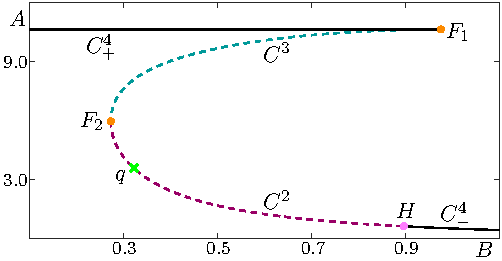
\includegraphics[]{./figures/MKMO_1.pdf}
\caption{Physically relevant branches $C^2$, $C^3$, $C^4_\pm$ of the critical manifold of (\ref{equation_1}) shown in projection onto the ($B$,$A$)-plane.  Branches $C^2$ (dashed, raspberry curve) and $C^3$ (dashed, teal curve) consist of saddles of (\ref{equation_2}) and $C^4_\pm$ (solid, black curve) consist of attractors of (\ref{equation_2}).  Superscripts indicate the number of stable directions possessed by a single equilibrium on a branch and subscripts are used to distinguish between the two branches of attractors.  Branches are divided by saddle-node bifurcation points $F_1$ and $F_2$ (orange dots) and a Hopf point $H$ (pink dot).  Also shown is a saddle equilibrium $q$ (green cross) of (\ref{equation_1}) existing on $C^2$.  Parameters are as in Table 1.}
\label{figure_1}
\end{figure}

The critical manifold $C$ in ($A$,$B$,$X$,$Y$)-space is divided into branches by bifurcation points of the fast subsystem (\ref{equation_2}), so that points on each branch have the same dimensions of stable and unstable eigenspaces.  In other words, the branches of $C$ are one-parameter families in $B$ of hyperbolic equilibria of system (\ref{equation_2}).  In our notation for branches, superscripts indicate the dimension in ($A$,$B$,$X$,$Y$)-space of the stable eigenspace of the branch, which are defined as the collection of stable eigenspaces of all the points on the branch.  The dimension of the stable eigenspaces of the branches is, hence, one plus than the dimension of the stable eigenspace of each point on the branch.  Further, we use subscripts to distinguish the two branches on which equilibria have three-dimensional stable eigenspaces; i.e. are attracting.  

Four branches of $C$ lie in the physically relevant region where all phase-space variables are positive, these are shown in Figure \ref{figure_1} in projection onto the ($B$,$A$)-plane.  The uppermost branch denoted $C^4_+$ (solid, black curve) consists of stable equilibria of (\ref{equation_2}).  It is separated from the branch of saddle equilibria denoted $C^3$ (dashed, teal curve), by a very sharp fold point $F_1$ (orange dot) at $B \approx 0.956$.  Folds in the critical manifold correspond to saddle-node bifurcations of system (\ref{equation_2}) with respect to the parameter $B$, these are points at which one of the real eigenvalues of the Jacobian evaluated at the point switches signs.  Another fold at $B \approx 0.273$ denoted $F_2$ (orange dot), separates $C^3$ from a lower branch of saddle equilibria denoted $C^2$ (dashed, raspberry curve).   The branch $C^2$ ends at a Hopf bifurcation $H$ (pink dot) at $B \approx 0.897$, where two complex-conjugate eigenvalues of the Jacobian pass through the imaginary axis of the complex plane.  To the right of $H$, there is again a stable branch of equilibria denoted $C^4_-$ (solid, black curve).

The point $q$ (green cross) on $C^2$ at $B \approx 0.323$ is an equilibrium of system (\ref{equation_3}) and is, hence, an equilibrium for the full system (\ref{equation_1}).  The equilibrium $q$ has a two-dimensional stable and two-dimensional unstable manifold that are denoted $W^s(q)$ and $W^u(q)$, respectively.  The manifolds $W^{s}(q)$ and $W^{u}(q)$ can be computed with the methods in \cite{Red_book} and are not shown in Figure \ref{figure_1}.  To the right of $W^u(q)$, in the ($B$, $A$)-projection, the flow is from right to left near $C^2$ in the full system (\ref{equation_1}).  To the left of $W^u(q)$, in the ($B$, $A$)-projection, the flow is from left to right near $C^2$.

Our interest is in the branches $C^3$ and $C^2$ because they are saddle objects of different type and are crucial for organising the phase space.  These branches of the critical manifold are invariant for $\varepsilon = 0$, but not for $\varepsilon > 0$.  However, they do persist as locally invariant manifolds called slow manifolds \cite{Fenichel}.  The associated slow manifolds are traditionally denoted by $S^3_\varepsilon$ and $S^2_\varepsilon$ but, for notational convenience, we drop the subscript indicating dependence on $\varepsilon$ and refer to these slow manifolds for $\varepsilon > 0$ simply as $S^3$ and $S^2$.  The slow manifold $S^3$ has the same dimension and stability and lies at an $O(\varepsilon)$ Hausdorff distance from $C^3$.  In particular, $S^3$ converges to $C^3$ as $\varepsilon \rightarrow 0$.  (For a definition of Hausdorff distance, see e.g. \cite{Hausdorff_Distance}.)  Orbit segments that lie on a slow manifold remain slow for $O(1)$ time with respect to the slow time scale.  It follows that any trajectory that remains slow for an $O(1)$ amount of slow time can be considered (to be on) a slow manifold.  However, eventually trajectories on a slow manifold may become fast. Due to their finite time nature, slow manifolds are not unique; however, any two slow manifolds lie exponentially close to each other in a suitable $O(\varepsilon)$ neighbourhood of $C$ \cite{Fenichel}.  To select a unique representative $S^3$ and $S^2$, we consider the slow manifold that remains slow for the longest amount of time.

The Stable Manifold Theorem tells us that each $p \in C^3$ has a stable and an unstable manifold that are tangent to and have the same dimensions as $E^{s}(p)$ and $E^{u}(p)$, respectively.  We denote the stable manifold of a point $p \in C^3$ by $W^{s}(p)$ and its unstable manifold by $W^{u}(p)$.  The manifolds $W^{s}(p)$ and $W^{u}(p)$ consist of trajectories in ($A$, $B$, $X$, $Y$)-space that converge to $p$ in forward and backward time respectively.  We can then define the collection of stable manifolds for $p \in C^3$ as $W^{s}(C^3) = \bigcup_{p \in C^3} W^{s}(p)$, which a three-dimensional manifold.  We can similarly define the three-dimensional unstable manifold $W^{u}(C^2)$ of $C^2$.

According to Fenichel Theory, for $\varepsilon > 0$, the manifold $W^{s}(C^3)$ also persists in an $O(\varepsilon)$ neighbourhood as a three-dimensional local stable manifold $W^{s}_{loc}(S^3)$ of $S^3$.  The local stable manifold $W^{s}_{loc}(S^3)$ consists of families of trajectories that have a fast approach to $S^3$ then remain close to $S^3$ for $O(1)$ slow time.  The global stable manifold $W^{s}(S^3)$ can be obtained by extending $W^{s}_{loc}(S^3)$ backwards in time.  The three-dimensional unstable manifold $W^{u}(S^2)$ associated with $S^2$ is similarly defined for backwards time.  Again, due to the finite-time nature of the definitions for the three-dimensional manifolds $W^{s}(S^3)$ and $W^{u}(S^2)$, they are not unique.  To select unique representatives, we consider two-parameter families of orbit segments that remain slow for the longest amount of time subject to boundary conditions described in further sections.  
 
 %Saddle slow manifold section   
 \section{Computation of saddle slow manifolds and their (un)stable manifolds}
    
The definition of a one-dimensional saddle slow manifold and its (un)stable manifolds are given in \cite{Saeed_Paper} which presents algorithms for their computation in a three-dimensional system.  We are going to define only a unique representative of $S^3$; the slow manifold $S^2$ can be defined in a similar manner.

\subsection{Definition of $S^3$}    
The precise definition of the slow manifold $S^3$ is given with respect to a closed interval $[B_{\mathrm{in}},B_{\mathrm{out}}]$ for the slow variable $B$.  The values for $B_{\mathrm{in}}$ and $B_{\mathrm{out}}$ are chosen such that $[B_{\mathrm{in}},B_{\mathrm{out}}] \subset [F_{1_B}, F_{2_B}]$.  Note that there is a segment in $C^3$ for which each point $p \in C^3$ is uniquely associated via its $B$-coordinate with a value $B_p \in [B_{\mathrm{in}},B_{\mathrm{out}}]$.  Hence, for each $B_p \in [B_{\mathrm{in}},B_{\mathrm{out}}]$ there is a unique point $p=(p_A,p_B,p_X,p_Y) \in C^3$ such that $p_B = B_p$.  In the three-dimensional subsection $\{ \begin{pmatrix} A & B & X & Y \end{pmatrix} \in \mathbb{R}^4 \; | \; B=p_B\}$ we define a solid three-sphere $D_\delta(B_p)$ with radius $\delta$ and centre $p$ , given formally by

\begin{equation*}
D_\delta(B_p)=\{w \in \mathbb{R}^4 \; | \; w_B = B_p, \left\lVert w-p \right\rVert \leq \delta\}.
\end{equation*}    
\noindent
The union 
\begin{equation*}
\mathscr{D} = \cup_{B_p \in [B_{\mathrm{in}}, B_{\mathrm{out}}]} D_\delta(B_p) 
\end{equation*}


\noindent
forms a four-dimensional compact cylinder.  The radius $\delta$ is small, but it needs to be at least of $O(\varepsilon)$ to ensure that $S^3$ lies in $\mathscr{D}$.  The one-parameter family of orbit segments that enter $\mathscr{D}$ via $D_\delta(B_{\mathrm{in}})$ and exit via $D_\delta(B_{\mathrm{out}})$ are candidates for $S^3$.   To select a unique representative $S^3$ that $S^3$ have maximal integration time in $\mathscr{D}$ while satisfying appropriate boundary conditions.  Our choice of boundary conditions is explained in section 3.2.
    
Figure \ref{figure_2} shows a sketch of the unique representative $S^3$ (green curve), in projection onto the $(B,A)$-plane.  Sketched in purple is $\mathscr{D}$ with the spheres $D_\delta(B_{\mathrm{in}})$ and $D_\delta(B_{\mathrm{out}})$ (purple disks) at either end.

\begin{figure}[!t]
\begin{center}
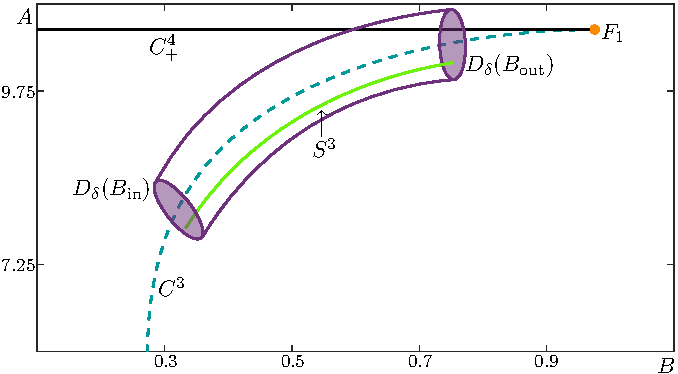
\includegraphics{./figures/MKMO_2.pdf}
\end{center}
\caption{A sketch of the unique representative slow manifold $S^3$ (green curve) projected into the ($B$,$A$)-plane.  The representative slow manifold $S^3$ is defined by having the longest integration time while entering and exiting  $D_\delta(B_{\mathrm{in}})$ and $D_\delta(B_{\mathrm{out}})$ (purple disks) at either end of a four-dimensional cylinder.  Also shown are $C^3$, $C^4_+$, and $F_1$.}
\label{figure_2}
\end{figure}

\subsection{Definition of $W^{s}(S^3)$ and computation of $W^{s}(S^3)$ and  $S^3$}

We define $W^{s}(S^3)$ to be a two-parameter family of orbit segments that enter into $\mathscr{D}$ at $D_{\delta}(B_p)$ for some $B_p \in [B_{\text{in}}, B_{\text{out}}]$, and remain inside $\mathscr{D}$ for $O(1)$ slow time.  We select and approximate a specific candidate for $W^{s}(S^3)$ by requiring that each orbit segment lying on $W^{s}(S^3)$ have maximal integration time inside $\mathscr{D}$ and satisfy boundary conditions outlined in the following paragraphs.  We now turn to the computation of the three-dimensional manifold $W^{s}(S^3)$ in the same region the two-dimensional stable manifold was investigated in the three-dimensional reduced model considered in \cite{QSSA}.
     
As $W^{s}(S^3)$ is three dimensional it is challenging to compute and difficult to visualise.  Examples of computing and visualising three-dimensional manifolds are in \cite{Initial_conditions_volume, Invariant_tori_again, Invariant_tori}.  None of these examples are in the context of computing (un)stable manifolds of saddle slow manifolds.  Tools to implement the computation of three-dimensional manifolds are not widely used at this time and, once computed, it is difficult to see the dynamics on the manifold in lower-dimensional projections.  Due to the nature of the current computation tools available, computing the entire three-dimensional manifold would also be computationally expensive compared to the the computation of two-dimensional manifolds.  A natural way forward is to consider a subset of $W^{s}(S^3)$ as a one-parameter family of two-dimensional submanifolds.  These can be computed by generalizing a method outlined in \cite{Saeed_Paper} which can then be implemented in the two-point boundary value problem (2PBVP) continuation package \textsc{Auto} \cite{AUTO}.  This is illustrated in Figure \ref{figure_2}.  A rigorous definition of a submanifold requires us to first define a two-dimensional plane $\Sigma$ that is transverse to the flow and $\bigcup_{p \in C^3} E^u(p)$ in our region of interest and is given by fixed values of $A$ and either $X$ or $Y$.  We approximate a submanifold with a smooth, one-parameter family of solutions to (\ref{equation_1}) with the property that they begin in $\Sigma$, enter $\mathscr{D}$ at $D_{\delta}(B_p)$ for some $B_p \in [B_{\text{in}}, B_{\text{out}}]$, and remain inside $\mathscr{D}$ for $O(1)$ slow time.  We use $W^{s}_{\Sigma}$ to denote the collection of those parts of the orbit segments that enter $\mathscr{D}$ in the fast direction.  The later parts that evolve mostly in the $B$-direction inside $\mathscr{D}$ for $O(1)$ slow time are considered to approximate parts of $S^3$.  If the later part of the orbit segment includes a fast exit from $\mathscr{D}$, that fast part is considered as an approximation of an orbit segment lying on the unstable manifold of $S^3$, $W^{u}(S^3)$.

Figure \ref{figure_3} illustrates, step-by-step, the algorithm for computing $W^s_\Sigma$ in projection onto ($B$, $A$)-space.  Panels (a)-(c) show first how to compute a specific submanifold $W^s_{\widehat{\Sigma}}$ for the plane $\widehat{\Sigma}$.  The plane $\widehat{\Sigma}$ is defined by the constant values $A \approx 10.6055$ and $Y \approx 0.000230006$.  These values are, respectively, the $A$- and $Y$-coordinates of the point $p_{\text{out}} \in C^3$ that has a $B$-coordinate value of $B_{\text{out}}=0.9$.  Panel (d) shows how to adjust the computation of $W^{s}_{\widehat{\Sigma}}$ for the computation of $W^{s}_\Sigma$ for a different plane, $\Sigma$.

\begin{figure}[h]
\centering
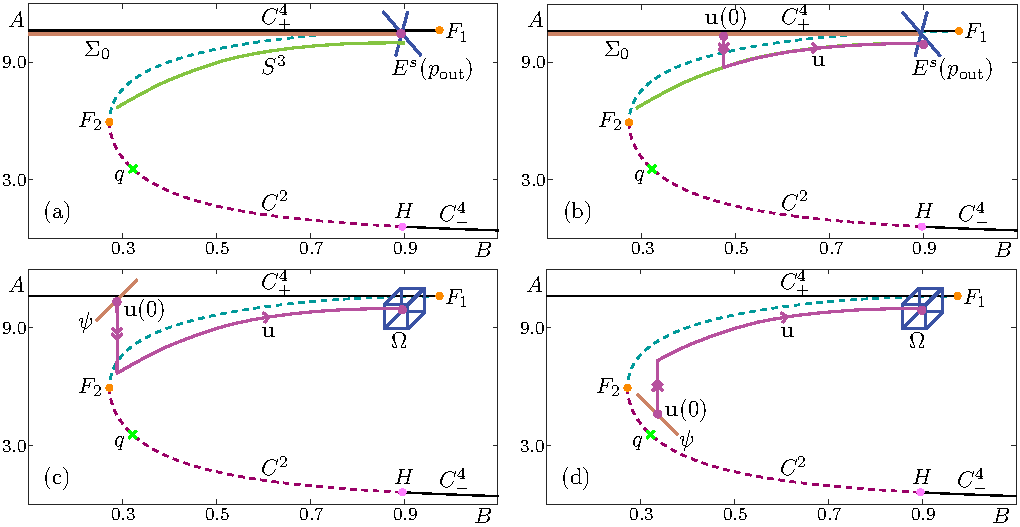
\includegraphics[]{./figures/MKMO_3.pdf}
\caption{A sketch of the numerical set-up for the computation of submanifolds of $W^s(S^3)$ in projection onto the ($B$,$A$)-plane.  Panel (a) shows a sketch at the start of the first homotopy step for computing $W^{s}_{\widehat{\Sigma}}$ with $S^3$ (represented by a green curve), $E^s(p_{\text{out}})$ (represented by a blue cross), and the plane $\widehat{\Sigma}$ (represented by a mocha line) which is defined by the $A$- and $Y$-coordinates of the point $p_{\text{out}}$.  Panel (b) shows a representative orbit segment $\mathbf{u}$ (represented by a magenta curve) of the first homotopy step.  Panel (c) shows an illustration of the selection of a $\mathbf{u}$ (represented by a magenta curve) with maximal integration time that starts at $\psi$ (represented by a mocha line) and ends on $\Omega$ (represented by a blue cube) which is spanned by $E^s(p_{\text{out}})$ and a vector in the $B$-direction; the one-dimensional subset $\psi \subset \widehat{\Sigma}$ is defined by fixing $B = B_{\text{in}}$.  Panel (d) shows a sketch of the selection of a different submanifold $W^{s}_{\Sigma}$ for $\Sigma$ on the other side of the critical manifold.  Also shown are $C^2$, $C^3$, $C^4_\pm$, $F_1$, $F_2$, $H$ and $q$.}
\label{figure_3}
\end{figure}


We compute the submanifold $W^s_{\widehat{\Sigma}}$ as a one-parameter family of orbit segments $\mathbf{u} = \{\mathbf{u}(s)| 0 \leq s \leq 1 \}$ of the rescaled system

\begin{equation}
\frac{d\mathbf{u}}{ds} = TF(\mathbf{u}),
\label{equation_4}
\end{equation}
    
\noindent
where $\mathbf{u}(s) = (A(s), B(s), X(s), Y(s)) \in \mathbb{R}^4$ is the vector of chemical concentrations, $F$ is the right-hand side of (\ref{equation_1}) and $T$ is the total integration time on the fast timescale, $t=Ts$.
    
Figure \ref{figure_3}(a) illustrates the set-up for obtaining a first solution on $W^s_{\widehat{\Sigma}}$ via a homotopy step.  Following the definition for $W^s_{\widehat{\Sigma}}$, we impose the condition
    
\begin{equation}
\mathbf{u}(0) \in \widehat{\Sigma}
\label{BC6}
\end{equation}
    
 \noindent
that is, we impose two restrictions on the startpoint of the orbit segment $\mathbf{u}$, $\mathbf{u}(0)$ because $\widehat{\Sigma}$ is two dimensional.  This boundary condition is illustrated in panel (a) where $\widehat{\Sigma}$ is sketched as a mocha, appearing directly under $C^4_+$.  As part of selecting a $\mathbf{u}$ that has a fast approach and remains close to $S^3$ (represented as a green curve in panel (a)) for $O(1)$ slow time, we consider the two-dimensional eigenspace $E^s(p^t_{\text{out}})$ that is transverse to $W^u(S^3)$.  We define the boundary condition
 
\begin{equation}
\mathbf{u}(1) \in E^s(p_{\text{out}})
\label{BC7}
\end{equation}
    
\noindent
that imposes two restrictions on the endpoint of $\mathbf{u}$, $\mathbf{u}(1)$ and allows for the possibility of $\mathbf{u}(1)$ intersecting $W^u(S^3)$.  This boundary condition is illustrated in panel (a) where $E^s(p^t_{\text{out}})$ is sketched as a blue cross.  The point $p_{\text{out}}$ is then a solution of the 2PBVP defined by (\ref{equation_4}), (\ref{BC6}) and (\ref{BC7}) with $T=0$.

Figure \ref{figure_3}(b) shows the next step where we increase the total integration time while allowing the $B$-coordinate value of $\mathbf{u}(0)$ to decrease towards $F_2$.  Note that increasing integration time in this fashion causes $T$ to become negative.  An intermediate orbit segment is represented as a magenta curve illustrating the presence of a fast segment (double arrows) followed by a slow segment (single arrow).  Panel (c) shows the stage at which the continuation is stopped, when $\mathbf{u}(0)_B = B_{\text{in}}=0.275$, just before $\mathbf{u}(0)_B$ reaches the $B$-coordinate value of $F_2$.
    
The orbit segment illustrated in Figure \ref{figure_3}(c) belongs to a two-parameter family of solutions $\mathbf{u}$ of (\ref{equation_4}) that satisfy the boundary conditions (\ref{BC6}) and (\ref{BC7}).  To select a one-parameter family of orbit segments from these, we select for each $B \in [B_{\text{in}}, B_{\text{out}}]$ the solution $\mathbf{u}$ with maximal integration time such that $\mathbf{u}(0)_B=B$.  To find an initial orbit segment satisfying this condition, we define the curve $\psi = \widehat{\Sigma}\cap \{ \omega \in \mathbb{R}^4 \; | \; \omega_B = B_{\text{in}}\}$, represented as a mocha line in panel (d), and require
    
    
\begin{equation}
\mathbf{u}(0) \in \psi,
\label{BCSTOP}
\end{equation}
    
\noindent
which imposes three conditions on $\mathbf{u}(0)$ and is more restrictive than (\ref{BC6}).  The boundary condition (\ref{BCSTOP}) is represented as a mocha line in Figure \ref{figure_3}(c).  Panel (c) also shows the three-dimensional space $\Omega$ spanned by the two stable eigenvectors of $p_{\text{out}}$ and $\begin{pmatrix} 0, & 1, & 0, & 0 \end{pmatrix}^{tr}$, represented as a blue cube.  Note that $\Omega$ is transverse to $\cup_{p \in C^3}E^u(p)$ and, hence, $W^u(S^3)$.  Instead of (\ref{BC7}) we require
    
\begin{equation}
\mathbf{u}(1) \in \Omega,
\label{BC11}
\end{equation}
    
\noindent
which imposes only one condition on $\mathbf{u}(0)$.  We now track the solution $\mathbf{u}$ of the 2PBVP (\ref{equation_4}), (\ref{BCSTOP}), (\ref{BC11}) as $T$ becomes more negative, forcing $\mathbf{u}(0)$ to approach $W^s(S^3) \cap \widehat{\Sigma}$ and $\mathbf{u}(1)$ to approach $W^u(S^3) \cap \Omega$. When a fold in $T$ is reached, a (local) minimum in the total integration time $T$ is attained.

The orbit segment that is obtained is not represented in a figure because it is almost identical to the orbit segment illustrated in Figure 3(c): it begins in $\widehat{\Sigma}$ and has a fast approach to $S^3$ before remaining $O(\varepsilon)$ close for $O(1)$ slow time, and so it lies on $W^{s}_{\widehat{\Sigma}}$ by definition.  In addition to finding an orbit segment that approximates a solution to (\ref{equation_4}) laying on $W^s_{\widehat{\Sigma}}$, we can approximate $S^3$ by restricting the orbit segment further inside $[B_{\text{in}},B_{\text{out}}]$ to exclude fast segments. At this stage the entire solution family lying on $W^s_{\widehat{\Sigma}}$ can be computed by continuing the fold in $T$, while allowing $u(0)_B$ to increase.

Panel (d) illustrates the case where we would like to compute $W^{s}_{\Sigma}$ where $\Sigma$ is defined by different constant values of $A$ and $Y$ (or $X$).  We can obtain a first orbit segment on $W^{s}_{\Sigma}$ via a second homotopy step after the first.  Using an intermediate orbit segment from the first homotopy step as a starting point, we impose (\ref{BC7}) while keeping as free parameters $T$, $\mathbf{u}(0)_B$, and the $X$-coordinate $\mathbf{u}(0)_X$ of $\mathbf{u}(0)$ (or the $Y$-coordinate  $\mathbf{u}(0)_Y$ of $\mathbf{u}(0)$).  In two runs, we continue $\mathbf{u}$ with $\mathbf{u}(0)_A$ and $\mathbf{u}(0)_Y$ (or $\mathbf{u}(0)_X$) as main continuation parameters.  In each of these runs, we increase or decrease the main continuation parameter until it attains the value necessary for $\mathbf{u}(0) \in \Sigma$.  Panel (d) shows an example of a $\mathbf{u}$ and $\psi$ corresponding to a choice of $\Sigma$ on the opposite side of the critical manifold from $\widehat{\Sigma}$ with respect to the $A$-coordinate.  Once $\mathbf{u}(0) \in \Sigma$, we follow the rest of the procedure described above while considering $\Sigma$ instead of $\widehat{\Sigma}$.

Figure \ref{figure_4} shows two projections of $W^s_{\widehat{\Sigma}}$ (light blue surface) with $\widehat{\Sigma}$ (mint surface).  Although the manifold is two dimensional, it is necessary to visualise it in both $(B,A,X)$- and $(B,A,Y)$-projections because it exists in four-dimensional space.  Lying on $W^s_{\widehat{\Sigma}}$ is a representative orbit segment, plotted in magenta.  The critical manifold is plotted and the view is rotated relative to earlier figures to help illustrate the geometry of the submanifold.  Orbits lying on $W^s_{\widehat{\Sigma}}$ have a fast approach to $S^3$ in $X$ and $Y$ before approaching mainly in the $A$-direction and then finally remaining close to $C^3$ for $O(1)$ slow time.

Figure \ref{figure_5} shows $W^s_{\widehat{\Sigma}}$ (light blue surface) together with one other submanifold $W^{s}_{\Sigma_1}$ (blue surface) of $W^{s}(S^3)$.  The additional submanifold was selected with $\Sigma_1$ (mint surface) given by $A=2.0$ and $Y=0.0$.  Figure \ref{figure_6} shows the two submanifolds of $W^{s}$ shown in Figure \ref{figure_5} along with three additional submanifolds (blue surfaces) and the planes $\Sigma$ (mint surfaces) that define them.  The additional submanifolds were selected with $\Sigma_2$ given by $A=4.0$ and $Y=0.75$, $\Sigma_3$ given by $A=4.0$ and $X=0.75$, and $\Sigma_4$ given by $A=6.0$ and $X=0.5$.  Note that the $\Sigma$ appear as lines in one of the two projections, depending on whether they are defined by constant values of $X$ or $Y$.  The submanifolds appear to intersect, however this is due to the variable $A$ being slower than variables $X$ and $Y$.  This causes orbit segments to approach $S^3$ in the $X$- and $Y$-directions before approaching in the $A$-direction and is the reason for the portions of the submanifolds that come very near to each other.  Different choices of $B_{\text{in}}$ and $B_{\text{out}}$ also cause some submanifolds to extend farther than others in the $B$-direction.

\begin{figure}[H]
\centering
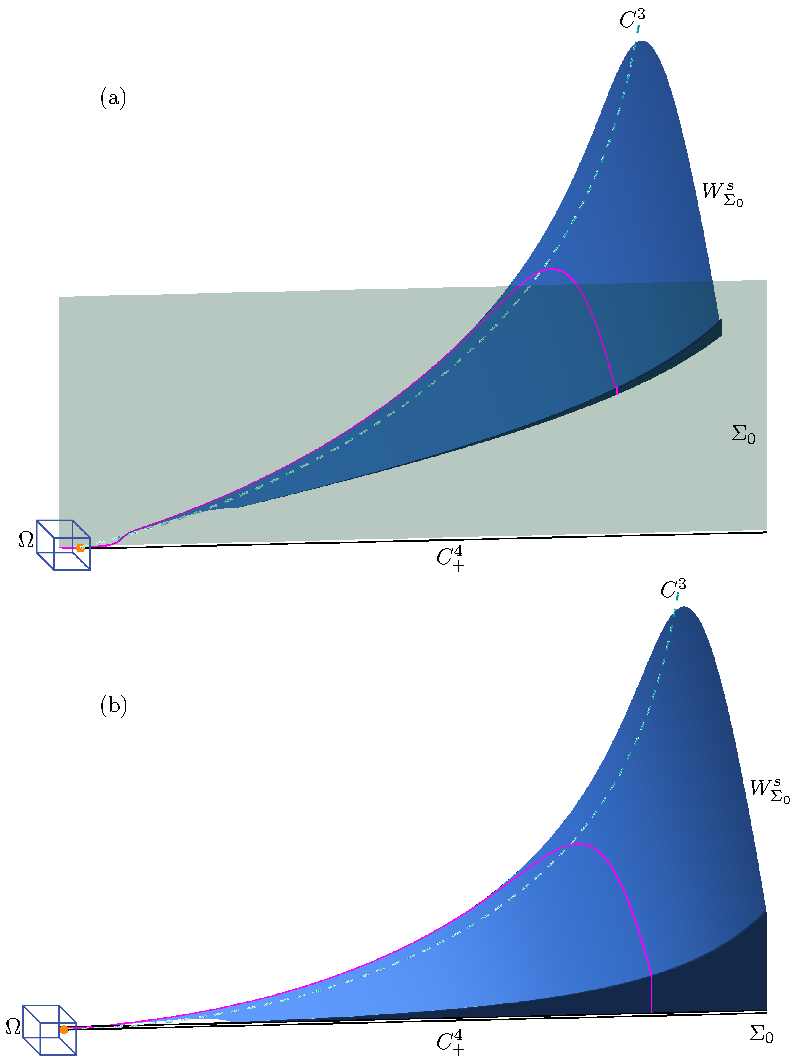
\includegraphics[]{./figures/MKMO_4.pdf}
\caption{The submanifold $W^{s}_{\widehat{\Sigma}}$ (light blue surface) of $W^s(S^3)$ shown in projection onto ($B$, $A$, $X$)-space (a) and onto ($B$, $A$, $Y$)-space (b) with a representative orbit segment (magenta curve), $\widehat{\Sigma}$ (mint surface and line), and $\Omega$ (represented by a blue cube).  Also shown are $C^3$, $C^4_+$, and $F_1$.  The view is rotated relative to previous figures.}
\label{figure_4}
\end{figure}



\begin{figure}[H]
\centering
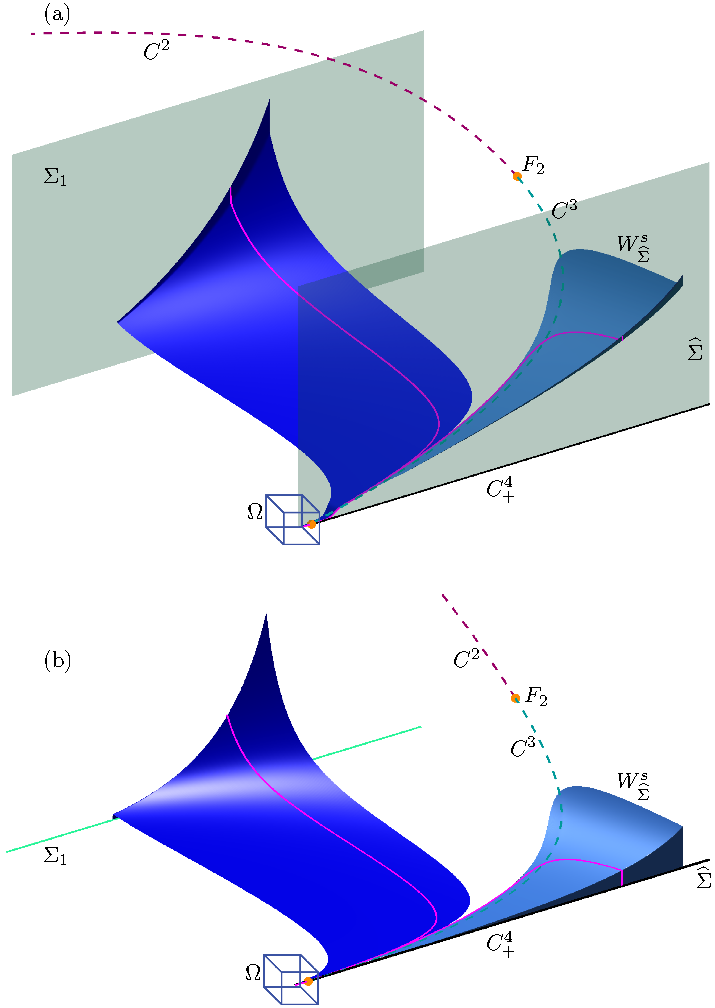
\includegraphics[]{./figures/MKMO_5.pdf}
\caption{The submanifolds $W^{s}_{\Sigma_1}$ (blue surface) and $W^{s}_{\widehat{\Sigma}}$ (light blue surface) of $W^s(S^3)$ shown in projection onto ($B$, $A$, $X$)-space (a) and onto ($B$, $A$, $Y$)-space (b) with representative orbit segments (magenta curves), planes $\widehat{\Sigma}$ (mint surface and line) and $\Sigma_1$ (mint surface and line), and $\Omega$ (represented by a blue cube).  Also shown are $C^2$, $C^3$, $C^4_+$, $F_1$, and $F_2$.}
\label{figure_5}
\end{figure}

\begin{figure}[H]
\centering
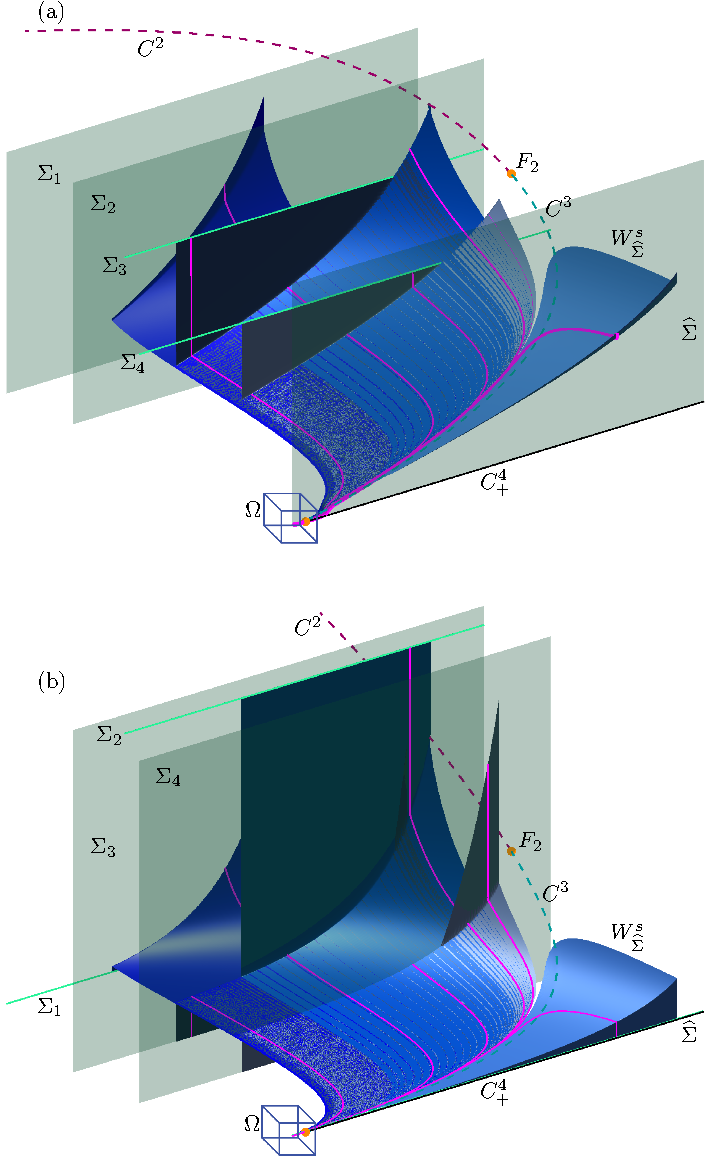
\includegraphics[]{./figures/MKMO_6.pdf}
\caption{The submanifolds from Figure 5. with three additional submanifolds $W^s_{\Sigma_i}$ (blue surfaces) defined by $\Sigma_2$, $\Sigma_3$, and $\Sigma_4$ (mint planes and lines) shown in projection onto ($B$, $A$, $X$)-space (a) and onto ($B$, $A$, $Y$)-space (b) with $\Omega$ (represented by a blue cube).  An example orbit segment (magenta curve) is plotted on each $W^s_{\Sigma_i}$.  Also shown are $C^2$, $C^3$, $C^4_+$, $F_1$, and $F_2$.}
\label{figure_6}
\end{figure}
    
We note that, unlike the stable manifold of $S^3$ computed for the reduced system in \cite{QSSA}, each submanifold $W^{s}_{\Sigma}$ in Figure \ref{figure_6} diverges backwards in time in the $X$- and $Y$- directions before reaching $S^2$.  The computations in \cite{QSSA} suggest that there exists a  submanifold of $W^s(S^3)$ in the four-dimensional system that spirals around $S^2$ in backward time for an appropriate choice of $\Sigma$.  Such a surface would be the intersection of the two three-dimensional manifolds $W^s(S^3)$ and $W^u(S^2)$ in the full four-dimensional system.  

%unstable
\subsection{Definition and computation of $W^{u}(S^2)$}  

Before investigating the existence of such an intersection, we first consider the unstable manifold $W^{u}(S^2)$ of $S^2$.  The computation of submanifolds of $W^{u}(S^2)$ is similar to the computation of $W^{s}_\Sigma$, however adjustments must be made in light of some complicating challenges.  Two extra challenges are the saddle equilibrium, $q$, of the full system lying on $C^2$ at $B = 0.323$ and the Hopf bifurcation of the fast subsystem at $B = 0.897$.  These are respectively shown as a green cross and a pink dot in Figures \ref{figure_1} and \ref{figure_3}.  Additional care must be taken to ensure that the computed orbits do not increase in integration time solely by approaching the saddle equilibrium's stable manifold or by following the stable slow manifold associated with $C^4_+$ backward in time.  Values for $B_{\mathrm{in}}$ and $B_{\mathrm{out}}$ are chosen such that $q_B < B_{\mathrm{out}} < B_{\mathrm{in}}< H_B$.  We can then define the four-dimensional cylinder $\mathscr{D}$ similarly to how it was defined for $W^s(S^3)$, substituting $C^2$ for $C^3$.  We consider a two-parameter family of orbit segments that enter $\mathscr{D}$ at $B_{\mathrm{in}}$, follow $S^2$ for an $O(1)$ amount of slow time and then exit at $B_p$ for some $B_p \in [B_{\mathrm{in}}, B_{\mathrm{out}}]$ and take the collection of fast, exiting segments of these to be $W^u(S^2)$.  We modify the steps for selecting and computing two-dimensional submanifolds of $W^s(S^3)$ in order to ensure that an increase in integration time results only from a more accurate approximation of a submanifold of $W^u(S^2)$.

To select a submanifold of $W^u(S^2)$, we first define for each $B_p \in [B_{\mathrm{in}}, B_{\mathrm{out}}]$ a sphere in the subspace $\{B=B_p\}$, centered at $p$ and with radius $r$; here $p \in C^2$ is the unique point such that $p_B = B_p$.  More formally,

\begin{equation*}
\widetilde{D}_r(B_p)=\{w \in \mathbb{R}^4 \;|\; w_B = B_p, \left\lVert w-p \right\lVert  = r\}.
\end{equation*}

\noindent
We can then define the three-dimensional cylinder $\mathscr{R} = \cup_{B \in [B_{\mathrm{in}}, B_{\mathrm{out}}]}\widetilde{D}_r(B)$.  

We select a submanifold $W^u_r$ for $r>\delta$, by taking a one-parameter family of orbit segments that enter $\mathscr{D}$ at $B_{\mathrm{in}}$ and, for each $B_p \in [B_{\mathrm{in}}, B_{\mathrm{out}}]$, intersect $\mathscr{R}$ after exiting $\mathscr{D}$ at $B_p$ an $O(1)$ amount of slow time afterwards.  To ensure that our choice of $W^u_r$ is unique, we require that orbit segments have maximal integration time for each $B_p \in [B_{\mathrm{in}}, B_{\mathrm{out}}]$.  The radius $r$ is chosen small enough so that $\mathscr{R}$ does not contain a locus of points at which the flow is not transverse to $\mathscr{R}$.  Using the cylinder $\mathscr{R}$ instead of the plane $\Sigma$ described in section 4.1 ensures that endpoints $\mathbf{u}(1)$ remain close enough to $C^2$ so that the $\mathbf{u}$ cannot contain segments that approach $q$.  In the following steps, the computation of a submanifold $W^u_{r^*}$ is outlined for $r^*=0.7$ before the description of the necessary modifications to obtain $W^u_r$ for more general $r$. 

We perform an initial homotopy step analogous to the first homotopy step in section 4.1 to obtain a first orbit segment that enters $\mathscr{D}$ at $B_{\mathrm{in}}$ and intersects $\mathscr{R}$ after exiting $\mathscr{D}$ at some $\tilde{B} \in [B_{\mathrm{in}}, B_{\mathrm{out}}]$.  We select the unique point $\tilde{p} \in C^2$ such that $\tilde{p}_B=0.7$.  The plane $\tilde{\Sigma}$ is defined by fixing the $A$- and $Y$- coordinates of $\tilde{p}$, which are $A \approx 0.940272$ and $Y \approx 1.342954$.  We impose the boundary conditions

\begin{equation}
\mathbf{u}(0) \in E^u(\tilde{p}),
\label{BC1_unstable}
\end{equation}

\noindent
and 

\begin{equation}
\mathbf{u}(1) \in \tilde{\Sigma}
\label{BC2_unstable}
\end{equation}
\noindent
which each impose two conditions on $\mathbf{u}(0)$ and $\mathbf{u}(1)$, respectively.  The point $\tilde{p}$ is then a solution to the 2PBVP defined by (\ref{equation_4}), (\ref{BC1_unstable}), and (\ref{BC2_unstable}) for $T=0$.  We increase $T$ while $\mathbf{u}(1)_B$ decreases and stop the continuation when $\mathbf{u}(1)$ intersects $\mathscr{R}$.  This step is almost identical to the initial homotopy step in section 4.1 except that we reverse the direction of time and instead of stopping the continuation when $\mathbf{u}(1)_B$ attains a certain value, we stop the continuation when $u(1)$ intersects $\mathscr{R}$.  We denote by $B_{\mathrm{stop}}$ the $B$-value of $\mathbf{u}(1)$ at the end of this step and $p^{\text{stop}}$ the corresponding point in $C^2$ such that $p^{\text{stop}_B}=B_{\text{stop}}$.

We perform a second homotopy step to ensure that $\mathbf{u}(0)$ is such that $\mathbf{u}$ can follow $S^2$ for $O(1)$ slow time while also ensuring that $\mathbf{u}$ cannot follow the attracting slow manifold for longer backward time.  In the second homotopy step we define a three-dimensional space $\Xi_{\textsc{hom2}}$ spanned by $E^u(\tilde{p})$ and a vector parallel to the $B$-direction.  We also define a one-dimensional circle $\Theta = \{ w \in \mathbb{R}^4 \; | \; w_Y=\bar{p}_Y, w_B=B_{\mathrm{stop}}, \left\lVert w-p^{\mathrm{stop}} \right\lVert=0.7\}$.  The orbit segment resulting from the first homotopy step is a solution to the 2PBVP defined by (\ref{equation_4}),

\begin{equation}
\mathbf{u}(0) \in \Xi_{\textsc{hom2}},
\label{BC3_unstable}
\end{equation}

\noindent
and 

\begin{equation}
\mathbf{u}(1) \in \Theta.
\label{BC4_unstable}
\end{equation}
\noindent
Our goal is to continue the orbit segment by increasing $T$ such that $u(0)_B$ increases, that is (\ref{BC3_unstable}) drives the continuation.  Condition (\ref{BC4_unstable}) is chosen such that integration time does not increase with decreasing $\mathbf{u}(1)_B$ and so that our 2PBVP is well defined.  The continuation is stopped when $\mathbf{u}(0)_B =1.0$.  The resulting orbit segment is initially attracted to the attracting slow manifold and follows it until it passes near $\mathscr{H}$ at which point $\mathbf{u}$ follows $S^2$.  As following the attracting slow manifold for longer backwards time requires the increase of $\mathbf{u}(0)_B$, we fix $\mathbf{u}(0)_B$ from this step onwards to prevent this from occurring.  This is different from section 4.1 in which $\mathbf{u}(1)_B$ remains free in the final steps of the computation (recall that we consider negative $T$ in section 4).

We define the plane $\Phi = \{w \in \Xi_{\textsc{hom2}} \; | \;  w_B=1.0\}$ and impose the boundary conditions

\begin{equation}
\mathbf{u}(0) \in \Phi,
\label{BC5_unstable}
\end{equation}

\noindent
and 

\begin{equation}
\mathbf{u}(1) \in \{ w \in \mathscr{R} \; | \; w_B=B_{\mathrm{stop}}\}.
\label{BC6_unstable}
\end{equation}
\noindent
Condition (\ref{BC6_unstable}) requires that $\mathbf{u}(1)$ remain on a two-dimensional sphere as opposed to the one-dimensional curve $\psi$ described for condition ($\ref{BCSTOP}$) in section 4.1.  We allow this extra degree of freedom for $\mathbf{u}(1)$ because keeping $\mathbf{u}(0)_B$ fixed in condition $(\ref{BC5_unstable}$) imposes an extra constraint compared to condition ($\ref{BC11}$) in section 4.1.  Our aim is to select a smooth, one-parameter family of orbit segments from the two-parameter family of orbit segments satisfying the 2PBVP defined by $(\ref{equation_4})$, ($\ref{BC5_unstable}$), and ($\ref{BC6_unstable}$).  To this end, for each $B_p \in [B_{\mathrm{in}},B_{\mathrm{out}}]$, we select from the one-parameter family of orbit segments exiting $\mathscr{D}$ at $B_p$ the orbit segment with maximal integration time.  The orbit segment resulting from the second homotopy step satisfies (\ref{equation_4}), ($\ref{BC5_unstable}$), and ($\ref{BC6_unstable}$).  To find an orbit segment with maximal integration time, we increase integration time until a fold in $T$ is detected.  The resulting orbit segment satisfies the conditions for being in $W^u_{r^*}$.  Finally to obtain the rest of the submanifold $W^u_{r^*}$ we switch the endpoint boundary condition to

\begin{equation}
\mathbf{u}(1) \in \mathscr{R}
\label{BC7_unstable}
\end{equation}
\noindent
which imposes one condition on $\mathbf{u}(1)$.  In two runs, the fold in $T$ is continued until $\mathbf{u}(0)_B=B_{\mathrm{out}}=0.35$ and then again until $\mathbf{u}(0)_B=B_{\mathrm{in}}=H_B$ to sweep out $W^u_{r^*}$.

Figure \ref{figure_7} shows two projections of the submanifold $W^u_{r^*}$ (red surface) with the curve of $\mathbf{u}(1)$ lying on $\mathscr{R}$ (mint curve) and $\phi$ (mint surface).  Two example orbit segments in $W^u_{r^*}$ (forest green curves) are plotted and a subset of $C^2$ (dashed raspberry curve) is shown.  To facilitate viewing, the view is rotated relative to previous figures.  From this angle, the radius of $\mathscr{R}$ may, to some readers, appear to approach $C^2$ with decreasing $\mathbf{u}(1)_B$.  This is due to the eye's erroneous association of points $\mathbf{u}(1)$ with points $p \in C^2$ such that $p_B < \mathbf{u}(1)_B$.

We can compute a different submanifold $W^u_r$ by returning to the second homotopy step in our computation.   Depending on the magnitude of $r$, we may need to perform one or two additional homotopy steps.  In the case where $r$ is large enough that $\widetilde{D}_r(\mathbf{u}(1)_B)$ contains a locus of points at which the flow is not transverse to it, an extra homotopy step is needed after the second.  We define a plane $\Xi_{\mathrm{hom3}}$ by fixing the $A$- and $X$-coordinates of $\mathbf{u}(1)$ after the second homotopy step.  To ensure that our 2PBVP is well defined, the orbit segment is continued with the boundary conditions (\ref{BC5_unstable}) and

\begin{equation}
\mathbf{u}(1) \in \Xi_{\mathrm{hom3}},
\label{BC8_unstable}
\end{equation}
\noindent
which imposes two conditions on $\mathbf{u}(1)$.  The endpoint $B$-coordinate $\mathbf{u}(1)_B$ is increased until $\widetilde{D}_r(\mathbf{u}(1)_B)$ no longer contains a locus of tangent points.

The final homotopy step involves defining another plane $\Xi_{\mathrm{homfinal}}$ by fixing the $B$- and $X$- values of $\mathbf{u}(1)$ after the second homotopy step, or the third homotopy step if a third homotopy step is necessary.  Condition (\ref{BC5_unstable}) is imposed while a new restriction

\begin{equation}
\mathbf{u}(1) \in \Xi_{\mathrm{homfinal}},
\label{BC9_unstable}
\end{equation}
\noindent
imposes two conditions on $\mathbf{u}(1)$.  The radius $r$ is then increased or decreased until the desired value is attained.  All that remains is to follow through with the rest of the steps to compute $W^u_r$.  In the last step, $B_{\text{out}}$ is chosen such that the flow is transverse to $\widetilde{D}(B_{\text{out}})$.  We do not show several submanifolds of $W^u(S^2)$ in the same figure, because the spiralling dynamics near $C^2$ make visualisation difficult in $(B,A,X)$-space and $(B,A,Y)$-space due to (self)-intersections of the submanifolds in these projections.

\begin{figure}[H]
\centering
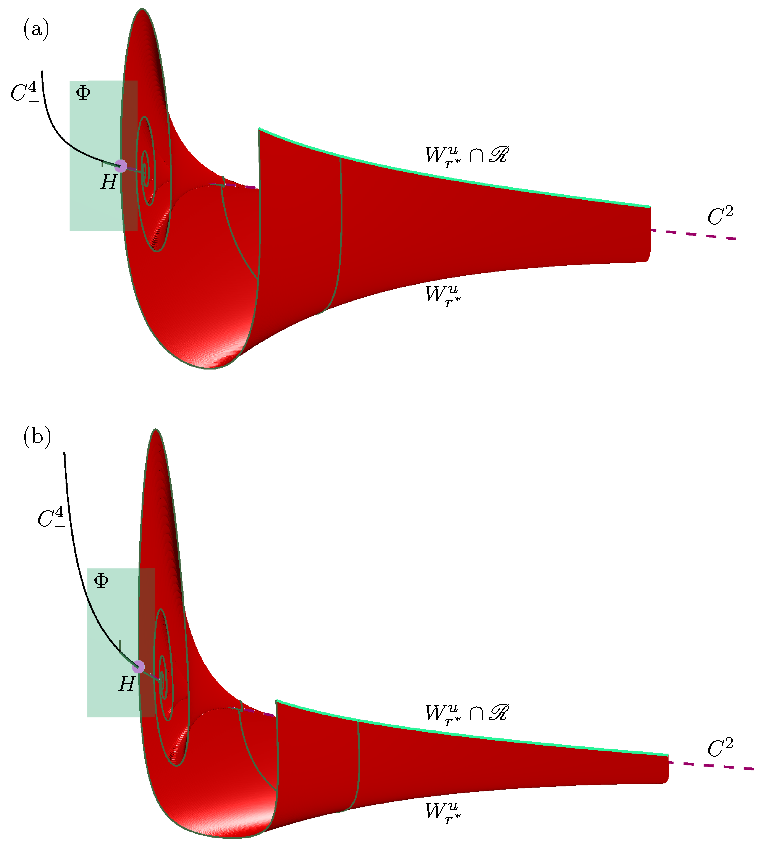
\includegraphics[]{./figures/MKMO_7.pdf}
\caption{The submanifold $W^u_{r^*}$ (red surface) of $W^u(S^2)$ shown in projection onto $(B,A,X)$-space (a) and $(B,A,Y)$-space (b); also shown are two representative orbit segments (forest green curves) on $W^u_{r^*}$, $\Phi$ (mint surface), and the intersection $W^s_{r^*}\cap\mathscr{R}$ (mint curve).  Branches $C^2$ and $C^4_-$ are also shown and the view is rotated relative to previous figures.  Also shown are $C^2$, $C^4_-$, and $H$.}
\label{figure_7}
\end{figure}


%Lin's method

\section{A heteroclinic connection between two saddle slow manifolds}

\begin{figure}[h]
\centering
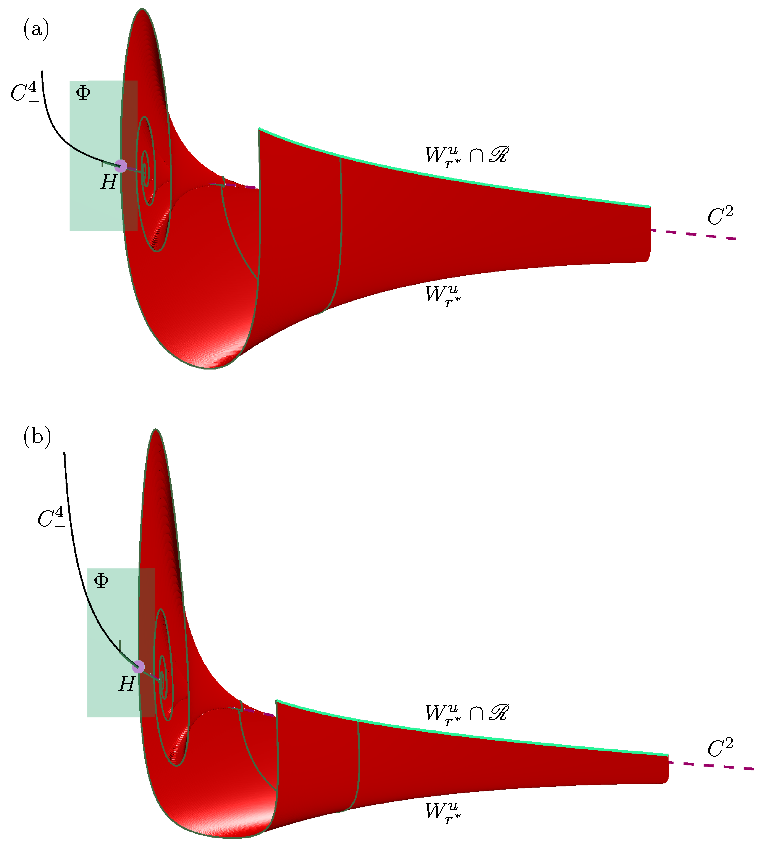
\includegraphics[]{./figures/MKMO_8.pdf}
\caption{Sketch of the numerical set up for the computation of $\mathscr{H}$ with Lin's method in projection onto the ($B$,$A$)-plane.  Panel (a) shows $S^2$ and $S^3$ (represented by green curves) and the Lin section $\mathscr{L}$ (represented by a charcoal line).  Panel (b) shows an initial orbit segment $\mathbf{u} \in W^s(S^3)$ (represented by a magenta curve) such that $\mathbf{u}(0) \in \mathscr{L}$ and $\mathbf{u}(1) \in E^s(p_{\text{out}})$ (represented by a blue cross).  Panel (c) additionally an initial orbit segment $\mathbf{w} \in W^u(S^2)$ (represented by a forest green curve) such that $\mathbf{w}(1) \in \mathscr{L}$ and $\mathbf{w}(0) \in E^u(p_{\text{in}})$ (represented by a red cross).  The points $\mathbf{u}(0)$, $\mathbf{w}(1)$ lie in the Lin space $Z \subset \mathscr{L}$ (represented by a gold line) at a distance $\eta$ (also represented by a gold line), called the Lin gap, from each other.  Also shown are $C^2$, $C^3$, $C^4_\pm$, $F_1$, $F_2$, and $H$.}
\label{figure_8}
\end{figure}


The two three-dimensional manifolds $W^s(S^3)$ and $W^u(S^2)$ are likely to intersect generically in a two-dimensional manifold of heteroclinic connections in the four-dimensional phase space [Is this a well-known enough fact not to reference it?].  We denote by $\mathscr{H}$ the surface of intersections to the right of $W^u(q)$ with respect to the $B$-coordinate in the ($B$, $A$)-projection.  We can compute such a surface of connections with an approach known as Lin's method \cite{Lin_original, Lin_POs, Lin_POs2}.  Since Lin's method is typically used in parameter continuation of heteroclinic connections that are not structurally stable, we explain the set-up here for our context.  Figure \ref{figure_8} illustrates the set-up step-by-step.  Panel (a) shows the critical manifold in projection onto ($B$, $A$)-space.  The three-dimensional so-called Lin section $\mathscr{L}$ (represented as a charcoal curve) is chosen so that it divides the four-dimensional phase space into two regions respectively containing $S^3$ (represented as a green curve) and $S^2$ (represented as a green curve) and so that, in the ($B$,$A$)-projection and with respect to the variable $A$, it lies between $q$ and the point on $C^3$ with the same $B$-coordinate as $q$.  Our choice of $\mathscr{L}$ allows us to avoid stopping the continuation because $\mathscr{L}$ has intersected $C^2$.  We can instead compute the largest possible portion of $\mathscr{H}$ by continuing orbit segments as close as possible to $q$.  In panel (b) we illustrate the computation of an orbit segment $\mathbf{u}$ (represented as a magenta curve) lying on $W^s(S^3)$ such that $\mathbf{u}(0) \in \mathscr{L}$.  Panel (c) additionally shows a representation of an orbit segment $\mathbf{w}$ (forest green curve) in $W^u(S^2)$ such that  $\mathbf{w}(1) \in \mathscr{L}$.

We define a vector $\mathbf{v}_Z \in \mathbb{R}^4$ called a Lin vector and given by 

	\begin{equation}
		\mathbf{v}_Z = \frac{\mathbf{u}(0) - \mathbf{w}(1)}{\left\lVert \mathbf{u}(0) - \mathbf{w}(1) \right\lVert}
		\label{Lin_vector}
	\end{equation}
	
\noindent	
as well as two unit normal vectors $\mathbf{n}_1, \mathbf{n}_2 \in \mathscr{L}$ such that $\mathbf{n}_i \perp \mathbf{v}_Z$ for $i=1,2$ and $\mathbf{n}_1 \perp \mathbf{n}_2$.  While our choice for the vector $\mathbf{v}_Z$, and normal vectors $\mathbf{n}_1$ and $\mathbf{n}_2$ is arbitrary, their selection remains fixed for the remainder of the computation.  The span of $\mathbf{v}_Z$ defines a one-dimensional space, $Z \subset \mathscr{L}$, called a Lin space and represented as a gold line in panel (c).  The distance between $\mathbf{u}(0)$ and $\mathbf{w}(1)$ in $Z$ defines the a Lin gap which is a regular test function which we denote $\eta$ and represent with the same gold line.  We approximate an orbit segment on $\mathscr{H}$ by continuation in the direction of decreasing $\eta$ while requiring $\mathbf{u}(0), \mathbf{w}(1) \in Z$.  When  $\eta = 0$, an orbit segment on $\mathscr{H}$ is detected as the concatenation of $\mathbf{w}$ and $\mathbf{u}$.

In our computations of $\mathbf{u}$ and $\mathbf{w}$ we do not search for orbit segments with maximal integration time as it is not straightforward to track two folds simultaneously with the automatic fold continuation in the package \textsc{Auto} \cite{AUTO}.  Since we are not requiring that $\mathbf{w}$ satisfy the condition of maximal integration time, we do not run into the same issues encountered in section 4.2 for the computation of a submanifold of $W^u(S^2)$.  For this reason we may compute $\mathbf{w}$ in a manner more similar to the computation of $\mathbf{u}$ in section~3.2.

\subsection{Computing an initial orbit segment on $W^s(S^3)$}

We choose $\mathscr{L} = \{\omega \in \mathbb{R}^4 \; | \; \omega_A = 6.0 \}$ and compute the orbit segment $\mathbf{u}$ as in the computation of an initial orbit segment on a submanifold $W^s_{\Sigma}$ in section~3.2 with the exception that we choose $B_{\text{out}}=0.95$ and omit last the step of computing the orbit with maximal integration time.  Here, $\Sigma$ is the plane given by $A=6.0$ and $Y=3.5072 \times 10^{-5}$ which is the $Y$-coordinate of our new $p_{\text{out}}$.

\subsection{Computing an initial orbit segment on $W^u(S^2)$}

We perform three homotopy steps to obtain an initial orbit segment on $W^u(S^2)$.  We begin with the point $\tilde{p}$ that is a solution to the 2PBVP defined by $(\ref{equation_4})$, (\ref{BC1_unstable}), and (\ref{BC2_unstable}) for $T=0$.  We obtain an orbit segment $\mathbf{w}$ by imposing conditions (\ref{BC1_unstable}) and (\ref{BC2_unstable}) while increasing integration time.  The continuation is stopped when $\mathbf{w}(1)_B = 0.6$.

We then impose (\ref{BC3_unstable}) and (\ref{BC2_unstable}) while additionally requiring $\mathbf{w}(1)_B=0.6$.  We continue $\mathbf{w}$ while increasing integration time once more while $\mathbf{w}(0)_B$ increases, and stop the continuation when $\mathbf{w}(0)_B=1.0$.

In the third homotopy step, we impose (\ref{BC5_unstable}) while keeping $\mathbf{w}(1)_B$ and $\mathbf{w}(1)_Y$ fixed.  The $A$-coordinate of $\mathbf{w}(1)$ increases as $T$ is increased.  The continuation is stopped when $\mathbf{w}(1)_A = 6.0$.  In other words, we stop the continuation when $\mathbf{w}(1) \in \mathscr{L}$.

\subsection{Closing the Lin gap}

We are now in a position to define vectors $\mathbf{v}_Z$, $\mathbf{n}_1$, and $\mathbf{n}_2$.  We define $\mathbf{v}_Z$ using the orbit segments $\mathbf{u}$ and $\mathbf{w}$ obtained in sections ~4.1 and ~4.2 and take $\mathbf{n}_1 = \begin{pmatrix} 0, & 0, & \mathbf{v}_{Z_Y}, & -\mathbf{v}_{Z_X} \end{pmatrix}^{tr}$, and $\mathbf{n}_2 = \begin{pmatrix} 0, & \mathbf{v}_{Z_Y}, & 0, & -\mathbf{v}_{Z_B} \end{pmatrix}^{tr}$.  We impose conditions

\begin{align}
	\begin{split}
		\mathbf{u}(0), \mathbf{w}(1) \in \mathscr{L},\\ \vspace{2mm}
		[\mathbf{u}(0) - \mathbf{w}(1)] \cdot \mathbf{n}_1 =0, \\ \vspace{2mm}
		[\mathbf{u}(0) - \mathbf{w}(1)] \cdot \mathbf{n}_2 =0
	\end{split}
	\label{Z}
\end{align}

\noindent
to restrict $[\mathbf{u}(0) -\mathbf{w}(1)] \in Z$ as illustrated in figure \ref{figure_8}(c).  Additionally, we impose conditions (\ref{BC7}) and (\ref{BC5_unstable}) while allowing the integration times of $\mathbf{u}$ and $\mathbf{w}$ to move freely.  As illustrated in panel (c), the pair of orbit segments $\mathbf{u}$ and $\mathbf{w}$ obtained at the end of section ~4.2 are one of a two-parameter family of orbit-segment pairs satisfying (\ref{BC7}), (\ref{BC5_unstable}), and (\ref{Z}).  To formulate a well-defined 2PBVP, we impose the restriction

\begin{equation}
\mathbf{w}(1)_B \in \{ \omega \in \mathbb{R}^4 \; | \; \omega_B = 0.6 \},
\label{fix_B}
\end{equation}  
\noindent
and continue $\mathbf{u}$ and $\mathbf{w}$ while $\eta$ is decreased.  We stop the continuation as soon as $\eta = 0$, at which point the concatenation of $\mathbf{w}$ with $\mathbf{u}$ forms an approximation of a heteroclinic connection in $\mathscr{H}$.

To obtain a one-parameter family of concatenations approximating $\mathscr{H}$, we require $\eta = 0$ while relaxing condition (\ref{fix_B}).  We then decrease $\mathbf{w}(1)_B$ and stop the continuation before $\mathbf{u}$ and $\mathbf{w}$ reach the intersection of $\mathscr{H}$ with $W^u(q)$.  We sweep out the other side of the manifold by continuation in the opposite direction (of increasing $\mathbf{w}(1)_B$) and stop just before $\mathbf{w}(1)_B$ reaches the $B$-coordinate of the Hopf bifurcation point $H$ on $C^2$.

Figure \ref{figure_9} shows $\mathscr{H}$ in projection onto ($B$,$A$,$X$)-space and ($B$,$A$,$Y$)-space with $\mathscr{L}$ (charcoal surface).  The surface of heteroclinic connections $\mathscr{H}$ is divided by $\mathscr{L}$ into a region composed of $\mathbf{w}$ (red surface) and a region composed of $\mathbf{u}$ (blue surface).  Three representative orbit segments are shown as concatenations of $\mathbf{w}$ (forest green curves) with $\mathbf{u}$ (magenta curves).  Orbit segments on $\mathscr{H}$ spiral around and follow $S^2$ for an $O(1)$ amount of slow time and then traverse the region between $C^2$ and $C^3$ to follow $S^3$ for an $O(1)$ amount of slow time.

\begin{figure}[H]
\centering
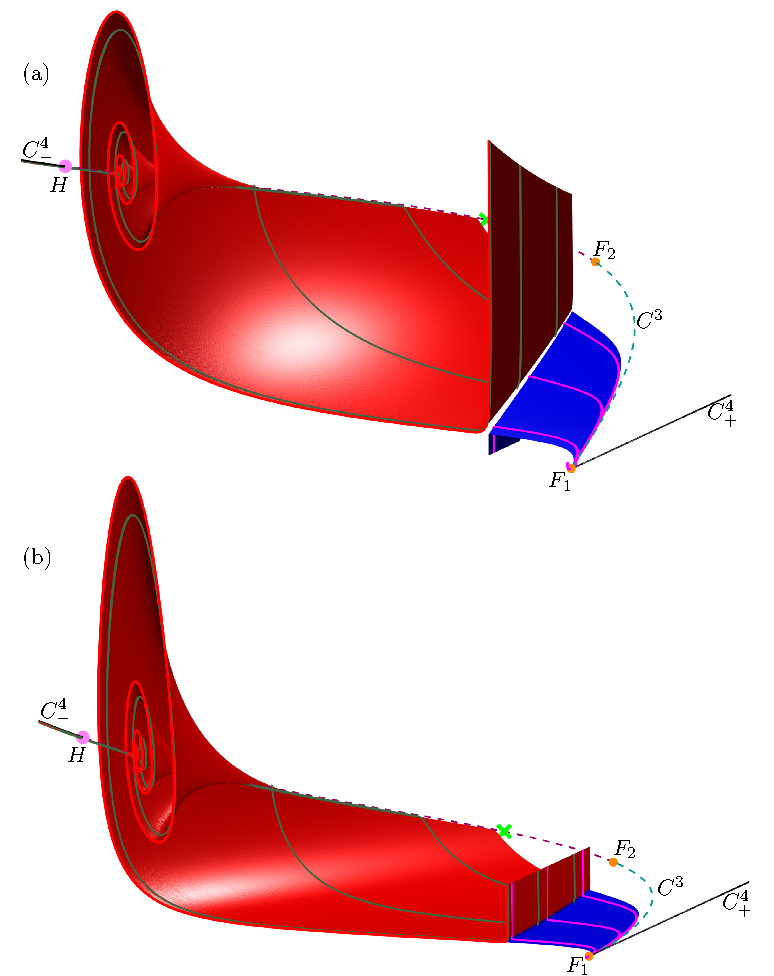
\includegraphics[]{./figures/MKMO_9.pdf}
\caption{The surface of heteroclinic connections $\mathscr{H}$ (red/blue surface) and the Lin section $\mathscr{L}$ (charcoal surface) in projection onto $(B,A,X)$-space (a) and onto $(B,A,Y)$-space (b).  The part of $\mathscr{H}$ that was computed as orbit segments in $W^s(S^3)$ is plotted in blue while the part that was computed as orbit segments in $W^u(S^2)$ is plotted in red.  Also shown are three representative orbit segments on $\mathscr{H}$, where the $\mathbf{u} \subset W^s(S^3)$ are magenta and the $\mathbf{w} \subset W^u(S^3)$ are forest green.  Notice the saddle equilibrium $q \in C^2$ (green cross) which is partially obstructed by $\mathscr{H}$ and $\mathscr{L}$.  Also shown are $C^2$, $C^3$, $C^4_\pm$, $F_1$, $F_2$, and $H$.}
\label{figure_9}
\end{figure}

Figure \ref{figure_10} shows $\mathscr{H}$ (red-blue fade surface) in projection onto ($B$, $A$, $X$)-space and ($B$, $A$, $X$)-space with the two-dimensional $W^u(q)$ (cardinal surface).  The unstable manifold $W^u(q)$ is shown bounding $\mathscr{H}$ and prevents us from computing the entire surface of heteroclinic connections.  It partially obstructs the saddle equilibrium $q$ (green cross).  Three representative orbit segments (forest green-magenta fade curves) are also shown originating from $S^2$ before traversing $\mathscr{H}$ to $S^3$.

\begin{figure}[H]
\centering
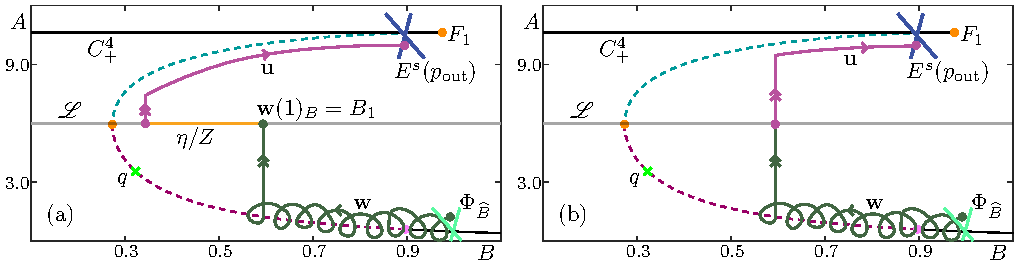
\includegraphics[]{./figures/MKMO_10.pdf}
\caption{The manifold $W^u(q)$ (cardinal surface) is shown in projection onto $(B,A,X)$-space (a) and onto $(B,A,Y)$-space (b) and bounds the computed surface of heteroclinic connections $\mathscr{H}$ (red-blue fade surface).  The saddle equilibrium $q$ (green cross) is partially obstructed by $\mathscr{H}$ and $W^{u}(q)$; compare with Figure 9.   Also shown are $C^2$, $C^3$, $C^4_\pm$, $F_1$, $F_2$, and $H$.}
\label{figure_10}
\end{figure}



%Singular surface computation

\section{Computing the singular surface of heteroclinic connections}

We compute the the singular surface analogous to $\mathscr{H}$, denoted $\mathscr{H}_0$, in the interest of analysing its interactions with MMOs for varying $\varepsilon$.  The computation of $\mathscr{H}_0$ for $\varepsilon=0$ is slightly different from the computation of $\mathscr{H}$ for $\varepsilon > 0$.  The time scaling parameter, $\varepsilon$, being zero means that $\mathscr{H}_0 = W^s(C^3) \cap W^u(C^2)$.  The surface $\mathscr{H}_0$ is then composed of the family of heteroclinic connections between saddle equilibria of (\ref{equation_2}) which is parameterized by $B$.  In ($B$,$A$)-space, the equilibria in $C^2$ to the left of $B \approx 0.476858$ with respect to the $B$-coordinate have all real eigenvectors.  Equilibria in $C^2$ to the right have a complex conjugate pair of eigenvectors.  Due to the change in the type of eigenvectors, we compute $\mathscr{H}_0$ in two pieces with two slightly different algorithms.  We first describe the computation for equilibria with real eigenvectors and then for equilibria with complex conjugate eigenvectors.  

For both computations, we consider solutions to the rescaled system

\begin{equation}
\frac{d\mathbf{u}}{ds} = TG(\mathbf{u}),
\label{fast_rescale}
\end{equation}

\noindent
where $\mathbf{u}(s) = (A(s), X(s), Y(s)) \in \mathbb{R}^3$ is the vector of chemical concentrations, $G$ is the right hand side of (\ref{equation_2}), and $T$ is integration time on the fast timescale $t=Ts$.  The Lin section $\mathscr{L}$ is again taken to be the space defined by a constant $A=6.0$.  Note that in the layer equation, $\mathscr{L}$ is two dimensional and $B$ is a parameter.

\subsection{Real eigenvalues}

For the first three steps of the computation, the parameter $B$ is kept constant at a value of $0.4$.  We compute an initial orbit segment on $W^{s}(C^3)$ following the algorithm for computing a two-dimensional global manifold as a solution family of BVPs outlined in \cite{Red_book}.  We consider the equilibrium $\tilde{p}_{\Re}$ of (\ref{equation_2}) for $B=0.4$ such that $\begin{pmatrix} \tilde{p}_{\Re_A},& 0.4,&\tilde{p}_{\Re_X},&\tilde{p}_{\Re_Y} \end{pmatrix} \in C^3$.  We define a plane $\widetilde{\Sigma}_{\Re} = \{ \omega \in \mathbb{R}^3  \; | \; \omega_Y = \tilde{p}_{\Re_Y} \}$ and a one-dimensional circle $\widetilde{\Gamma}_{\Re}= \{ \omega \in \mathbb{R}^3  \; | \; \tilde{p}_{\Re} + r_{\Re}(\mathbf{v}_1\sin(\theta) + \mathbf{v}_2\cos(\theta)), \theta \in [0,2\pi) \}$  where $r_{\Re}=0.0001$ and $\mathbf{v}_1$ and $\mathbf{v}_2$ are the stable eigenvectors of $\tilde{p}_{\Re}$.  The radius $r_{\Re}$ of $\widetilde{\Gamma}_{\Re}$ is chosen small enough that $\widetilde{\Gamma}_{\Re}$ approximates a curve lying on $W^{s}(\tilde{p}_{\Re})$ and large enough that $\textsc{Auto}$ can distinguish points on $\widetilde{\Gamma}_{\Re}$ from $\tilde{p}_{\Re}$.  The point $\tilde{p}_{\Re} + r_{\Re}\mathbf{v}_2$ is then a solution to the 2PBVP defined by (\ref{fast_rescale}) and the conditions

\begin{equation}
	\mathbf{u}(1) \in \widetilde{\Gamma}_{\Re},
	\label{top_end}
\end{equation}

and

\begin{equation}
	\mathbf{u}(0) \in \widetilde{\Sigma}_{\Re}
\end{equation}

\noindent
for $T=0$.  An initial orbit segment, $\mathbf{u}$, on $W^{s}(C^3)$ with start point in $\mathscr{L}$ is obtained by decreasing $\mathbf{u}(0)_A$ while also allowing integration time to increase in backwards time, corresponding to negative $T$.  The continuation is stopped when $\mathbf{u}(0) \in \mathscr{L}$, in other words, when $\mathbf{u}(0)_A = 6.0$.

In the second step, we obtain an initial orbit segment on $W^{u}(C^2)$ with end point in $\mathscr{L}$ through almost identical means.  We consider the equilibrium $\hat{p}_{\Re}$ of (\ref{equation_2}) for $B=0.4$ such that $\begin{pmatrix} \hat{p}_{\Re_A}, &0.4, & \hat{p}_{\Re_X}, & \hat{p}_{\Re_Y} \end{pmatrix} \in C^2$ and the unstable eigenvectors $\mathbf{k}_1$ and $\mathbf{k}_2$ of $\hat{p}_{\Re}$.  We then define $\widehat{\Gamma}_{\Re} = \{ \omega \in \mathbb{R}^3  \; | \; \tilde{p}_{\Re} + r_{\Re}(\mathbf{v}_1\sin(\theta) + \mathbf{v}_2\cos(\theta)), \theta \in [0,2\pi) \}$.  The point $\hat{p}_{\Re} + r_{\Re}\mathbf{k}_2$ is then a solution to the 2PBVP defined by (\ref{fast_rescale}) and the conditions

\begin{equation}
	\mathbf{w}(0) \in \widehat{\Gamma}_{\Re}
	\label{bottom_start}
\end{equation}

and

\begin{equation}
	\mathbf{w}(1) \in \widehat{\Sigma}_{\Re},
\end{equation}

\noindent
for $T=0$.  We increase $\mathbf{w}(1)_A$ while also allowing integration time to increase in forward time, corresponding to positive $T$.  The continuation is stopped when $\mathbf{w}(1) \in \mathscr{L}$.

In the third step, we define the Lin vector 

\begin{equation}
	\mathbf{v}_Z = \frac{\mathbf{u}(0) - \mathbf{w}(1)}{\left\lVert \mathbf{u}(0) - \mathbf{w}(1) \right\lVert},
	\label{Lin_vector_singular}
\end{equation}

\noindent
that is three dimensional.  We also define a normal vector $\mathbf{n} = \begin{pmatrix} 0, & -\mathbf{v}_{Z_Y}, &-\mathbf{v}_{Z_X} \end{pmatrix}$ such that $\mathbf{n} \perp \mathbf{v}_Z$.  We then define the conditions 

\begin{align}
	\begin{split}
		\mathbf{u}(0), \mathbf{w}(1) \in \mathscr{L} \\ \vspace{2mm}
		\begin{pmatrix}\mathbf{u}(0) - \mathbf{w}(1)\end{pmatrix} \cdot \mathbf{n} =0.
	\end{split}
	\label{singular_Z}
\end{align}

\noindent
To close the Lin gap, $\eta$ we impose conditions (\ref{top_end}), (\ref{bottom_start}), and (\ref{singular_Z}) while decreasing $\eta$ and allowing integration time to move freely.  The continuation is stopped when $\eta = 0$ at which point the concatenation of $\mathbf{w}$ with $\mathbf{u}$ forms an approximation of a heteroclinic connection on $\mathscr{H}_0$.  We can then sweep out the portion of $\mathscr{H}_0$ corresponding to real eigenvalues increasing and decreasing the parameter $B$ inside the interval ($F_{2_B}$, 0.47685750162] while requiring that $\eta=0$.  We choose to stop our continuation at $B = 0.47685750162$, before the eigenvalues switch from real to complex conjugate.  Unlike the computation of $\mathscr{H}$, the computational set up for $\mathscr{H^*}$ allows us to decrease $B$ past the value of $q_B$.  We are thus able to compute the entire portion of $\mathscr{H}_0$ corresponding to real eigenvalues.

\subsection{Complex conjugate eigenvalues}

The method for computing an initial orbit segment, $\mathbf{u}$, on $W^{s}(C^3)$ for complex conjugate eigenvalues is similar except that throughout the computation and the definitions of associated surfaces, we substitute $\tilde{p}_{\Re}$ for the equilibrium $\tilde{p}_{\Im}$ of \ref{equation_2} for $B=0.7$ such that $\begin{pmatrix}\tilde{p}_{\Im_A}, &0.7, &\tilde{p}_{\Im_X}, &\tilde{p}_{\Im_Y} \end{pmatrix}$.

The computation of orbit segments on $W^u(C^2)$ for $B$-values whose corresponding equilibria on $C^2$ that have complex conjugate eigenvalues presents the additional challenge.  Namely, some orbit segments on $W^u(C^2)$ contain a segment that spirals tightly around $C^2$ while others do not.  Orbit segments that spiral require larger mesh sizes than those that do not, however mesh size is held constant in our continuation.  To address this issue, we define a radius $r_{\Im} =  f(B)$, where $f(B)$ is the linear function such that $f(0.47685750164)=0.0001$ and $f(0.86)=0.2$.  This allows us to avoid the tightly spiralling regions by choosing a start point farther away from $C^2$ in those areas.

To compute an initial orbit segment, $\mathbf{w}$, on $W^u(C^2)$, we begin by considering the equilibrium $\hat{p}_{\Im}$ of (\ref{equation_2}) for $B=0.7$ such that $\begin{pmatrix} \hat{p}_{\Im_A},& 0.7,&\hat{p}_{\Im_X},&\hat{p}_{\Im_Y} \end{pmatrix} \in C^2$.  $\widehat{\Sigma}_{\Im} = \{ \omega \in \mathbb{R}^3  \; | \; \omega_Y = \hat{p}_{\Im_Y} \}$ and a one-dimensional circle $\widehat{\Gamma}_{\Re}= \{ \omega \in \mathbb{R}^3  \; | \; \hat{p}_{\Im} + f(0.7)(\mathbf{h}_1\sin(\theta) + \mathbf{h}_2\cos(\theta)), \theta \in [0,2\pi) \}$  where $\mathbf{h}_1$ and $\mathbf{h}_2$ are the real and complex parts of the unstable complex conjugate eigenvectors of $\hat{p}_{\Re}$.  The point $\hat{p}_{\Im} + f(0.7)\mathbf{h}_2$ then becomes a solution to the 2PBVP defined by (\ref{fast_rescale}) and the conditions

\begin{equation}
	\mathbf{w}(0) \in \widehat{\Gamma}_{\Im}
	\label{bottom_start_complex}
\end{equation}

and

\begin{equation}
	\mathbf{w}(1) \in \widehat{\Sigma}_{\Im},
\end{equation}

\noindent
for $T=0$.  To obtain a $\mathbf{w}$ such that $\mathbf{w}(1) \in \mathscr{L}$, we increase $\mathbf{w}(1)_A$ while allowing $T$ to increase and stop the continuation when $\mathbf{w}(1)_A=6.0$.

We close the Lin gap by imposing the conditions (\ref{top_end}), (\ref{Lin_vector_singular}), and (\ref{bottom_start_complex}) while decreasing $\eta$ and allowing integration to move freely.  The continuation is stopped when $\eta=0$ at which point the concatenation of $\mathbf{w}$ with $\mathbf{u}$ forms an approximation of a heteroclinic connection on $\mathscr{H}_0$.  We can then sweep out the portion of the manifold corresponding to complex conjugate eigenvalues by increasing and decreasing the parameter B inside the interval $[0.47685750164, H)$ while requiring that $\eta=0$.  We choose to stop the continuation at $B=0.47685750164$ before the eigenvalues switch from complex conjugate to real.

\begin{figure}[H]
\centering
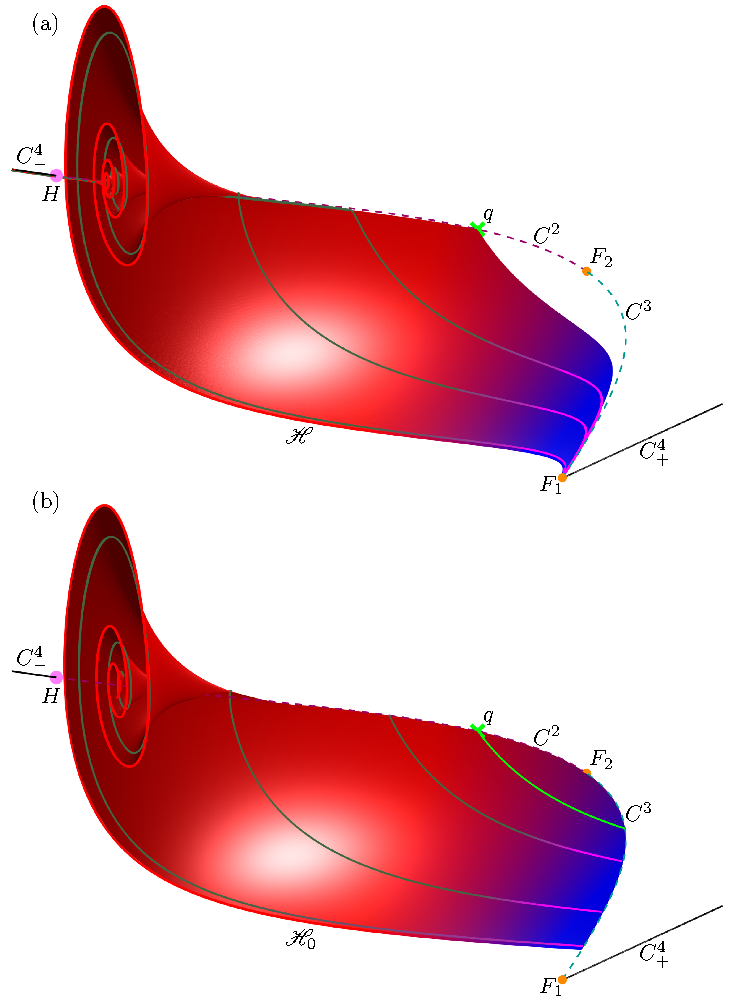
\includegraphics[]{./figures/MKMO_11.pdf}
\caption{Projections onto ($B$, $A$, $X$)-space of $\mathscr{H}$ (red-blue fade surface) (a) and of the portion of $\mathscr{H}_0$ (red-blue fade surface) lying in the region $B < 0.781$ (b) with representative orbit segments (forest green-magenta fade curves).  Also shown are the intersection $W^u(q)\cap\mathscr{H}_0$ (green curve) for $\varepsilon=0$, $q$, $C^2$, $C^3$, $C^4_\pm$, $F_1$, $F_2$, and $H$.}
\label{figure_11}
\end{figure}

Figure \ref{heteroclinic_singular} shows $\mathscr{H}_0$ projected into ($B$,$A$,$X$)- and ($B$,$A$,$Y$)-space.  For visual comparison with $\mathscr{H}$, we show only the portion of $\mathscr{H}_0$ that lies in the region $B < 0.781$.  The computational set up is not visualized in figure \ref{heteroclinic_singular} and the color of $\mathscr{H}_0$ fades from red to blue in colouring to illustrate its non-dependence on our choice of $\mathscr{L}$.

\subsection{Distance from $\mathscr{H}_0$}

We analyse the difference between $\mathscr{H}$ and $\mathscr{H}_0$ using the integral norm to measure the distance between intersection curves of $\mathscr{H}$ and $\mathscr{H}_0$ with different subspaces of the phase space defined by constant values of $B$.


%%MMO section
\section{Implications for mixed-mode oscillation geometry}


\begin{figure}[H]
\centering
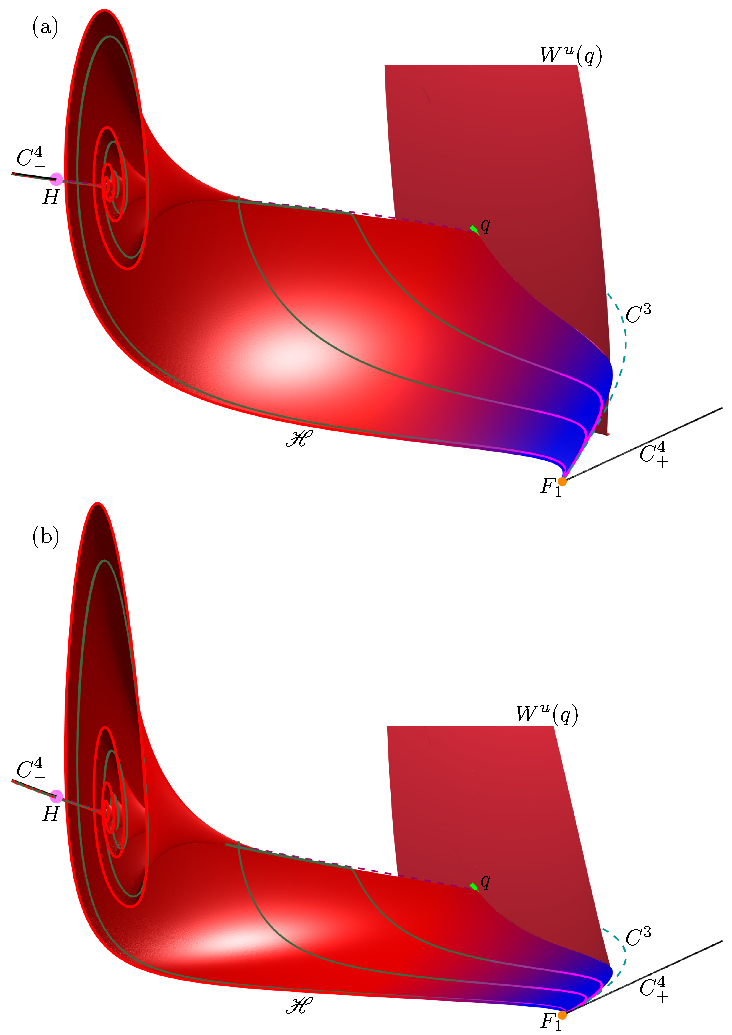
\includegraphics[]{./figures/MKMO_12.pdf}
\caption{The isola of MMO $\Gamma$ over $\varepsilon$.  The PO $\Gamma$ is stable along the blue part and unstable along the red part of the isola.  Green dots labeled (a), (b), and (c) correspond to $\Gamma$ as shown in Figure 14.}
\label{figure_12}
\end{figure}

\begin{figure}[H]
\centering
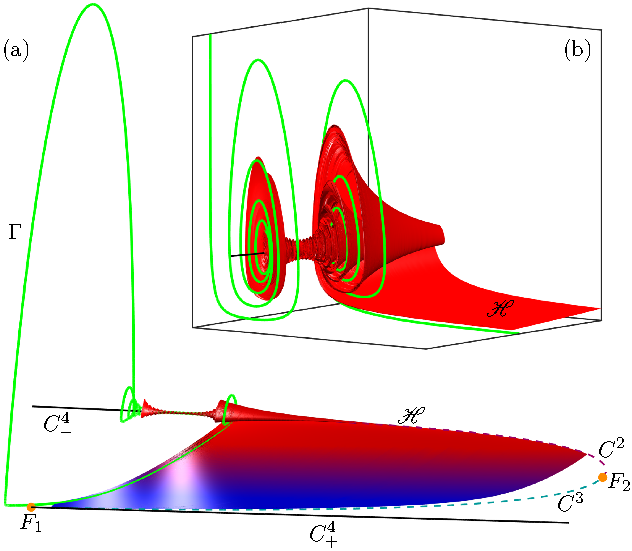
\includegraphics[]{./figures/MKMO_13.pdf}
\caption{The MMO $\Gamma$ (green curve) and the surface of heteroclinic connections $\mathscr{H}$ (red-blue fade) extended in backwards time past the Hopf bifurcation point $H$ are shown in projection onto ($B$,$A$,$X$)-space.  Panel (a) shows the global view of $\Gamma$ tracking $\mathscr{H}$ from $C^2$ to $C^3$ and making a LAO to $C^4_-$.  Panel (b) shows the subsequent slow passage of $\Gamma$ through $H$.  Also shown are $q$, $C^2$, $C^3$, $C^4_\pm$, $F_1$, $F_2$, and $H$.}
\label{figure_13}
\end{figure}

\begin{figure}[H]
\centering
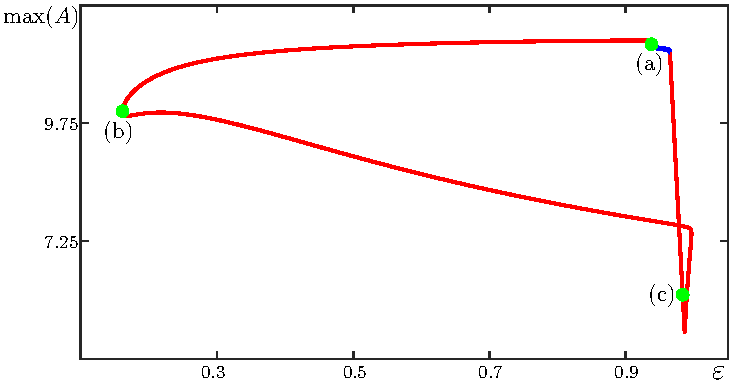
\includegraphics[]{./figures/MKMO_14.pdf}
\caption{Projections onto ($B$, $A$, $X$)-space of the portion of $\mathscr{H}_0$ (red-blue fade surface) lying in the region $B<0.781$, of the jump back trajectory $\mathscr{J}$ (magenta curve) and its dual $\mathscr{J}^*$ (magenta curve), and of the surface of singular POs $\mathscr{P}$ (midnight grape surface).  Also shown are $C^2$, $C^3$, $C^4_\pm$, $F_1$, $F_2$, and $H$.  Panel (a) shows $\Gamma$ (green curve) for the orignal value of $\varepsilon$.  The entry and exit of $\Gamma$ into the region of SAOs are near $\mathscr{J}$ and $\mathscr{J}^*$, respectively.  Panel (b) shows shows a representative $\Gamma$ (green curve) that remains near $\mathscr{P}$.  Panel (c) shows a representative $\Gamma$ (green curve) that has two LAOs.  Entry and exits into the region of SAOs are again near $\mathscr{J}$ and $\mathscr{J}^*$, respectively.}
\label{figure_14}
\end{figure}

We investigate the interaction between the MMO and $\mathscr{H}$ and $\mathscr{H}_0$ respectively for varying $\varepsilon$.  We consider the original MMO of interest corresponding to the original value $\varepsilon=0.0037$ as well as MMOs corresponding to $\varepsilon=0.0038$ and $\varepsilon=0.0005$.  These are representative MMOs of different type within the MMO parameter regime.  For the original MMO, we consider the effect of the surface $\mathscr{H}$ and then explore the singular objects, including $\mathscr{H}_0$, that also affect the geometry.  For the MMOs corresponding to $\varepsilon=0.0038$ and $\varepsilon=0.0005$ we only consider the singular objects that organize the MMO geometry.  Our analysis in section 5.3 shows that the difference between $\mathscr{H}$ and $\mathscr{H}_0$ is minimal and so it is reasonable to only consider $\mathscr{H}_0$ for MMOs corresponding to small $\varepsilon$.

Figures \ref{MMO_hetclin}(a) and (b)  show ($B$,$A$,$X$)- and ($B$,$A$,$Y$)-projections of the mixed-mode oscillation, neon green, plotted with $\mathscr{H}$, red to blue fade.  In this figure, we have extended $\mathscr{H}$ so that $\mathbf{u}(0)_B = \mathbf{w}(1)_B = 0.8724$. This facilitates comprehension of the MMO's entry into the region of SAOs, although it obscures some of the geometry of $\mathscr{H}$.  The surface serves as a reinjection mechanism from the region of SAOs into the region of LAOs.  The MMO begins near $C^4_-$ and spirals as it passes through the $H$ point to $C^2$.  The distance in $B$ between $H$ and the MMO's exit from the region of SAOs is approximately the same as the distance in $B$ between the MMO's entry and $H$.  After exiting the region of SAOs, the MMO traverses $\mathscr{H}$ to reach $C^3$.  The MMO follows $C^3$ and then makes a large, fast excursion mostly in the $X$ and $Y$ directions before being attracted back to $C^4_-$ again.  Shown in the inlays are enlargements of the region of SAOs.  In these enlargements, we see the details of the scrolling region of $\mathscr{H}$ and the slow passage of the MMO through the Hopf bifurcation.

Figure \ref{MMO1}(a) and (b) show ($B$,$A$,$X$)- and ($B$,$A$,$Y$)- projections of an enlargement of the original MMO with several singular objects.  The singular surface of heteroclinic connections $\mathscr{H}_0$ is plotted fading from red to blue.  The jump back trajectory, plotted in magenta, is the trajectory in \ref{equation_2} that connects $F_1$ to the equilibrium of (\ref{equation_2}) for $B=F_{1_B}$ lying on $C^4_-$.  The jump trajectory's dual is the trajectory lying on $\mathscr{H}_0$ that is at the same distance from $H$ with respect to $B$ as the jump trajectory.  A surface of saddle periodic orbits (POs) of system (\ref{equation_2}) is plotted in midnight grape.  These originate from $H$ and terminate in a homoclinic connection of an equilibrium of (\ref{equation_2}) lying on $C^3$.  The MMO's entry into and exit from the region of SAOs remain close to the jump orbit and it's dual respectively.  A significant amount of drift in the $B$ direction can be seen in the MMO away from the slow manifolds.  Figure \ref{MMO1}(c) shows an isola in parameter space that the MMO lies on.  The horizontal axis indicates the value of $\varepsilon$ and the vertical axis indicates the maximum value of the variable $A$ on the MMO.  Red curves indicate where the MMO has at least one unstable Floquet multiplier while blue curves indicate where the MMO is stable.  The location of the MMO on the isola is indicated with a green dot and signifies that the original MMO is stable.

Figure \ref{MMO2}(a) and (b) show ($B$,$A$,$X$)- and ($B$,$A$,$Y$)-projections of a zoom of the MMO for $\varepsilon=0.0005$ with the singular objects described above.  The MMO, plotted in neon green, remains close to the surface of singular POs.  The MMO enters the region of SAOs via the homoclinic connection of the equilibrium lying on $C^3$ and the SAOs track the interior of the surface of singular POs in the ($B$,$A$,$X$)- and ($B$,$A$,$Y$)- projections.  The MMO exits the region of SAOs by passing through the surface of singular POs in the ($B$,$A$,$X$)- and ($B$,$A$,$Y$)-projections and then being repelled away from it.  Figure \ref{MMO2}(a) shows the location of the MMO on the leftmost fold of the isola.

Figure \ref{MMO3}(a) and (b) show ($B$,$A$,$X$)- and ($B$,$A$,$Y$)-projections of a zoom of the MMO for $\varepsilon=0.0005$ with the singular objects described above.  Similarly to the MMO at $\varepsilon=0.0037$, the SAOs for the MMO at $\varepsilon = 0.0038$ are due to a slow passage through $H$.  The entry and exits from the region of SAOs are close to the jump trajectory and its dual.  An early return to $C^2$ occurs between the MMO's exit and reentry into the region of SAOs.  This MMO differs from the other MMOs discussed as it has two LAOs instead of one.  Figure \ref{MMO3}(c) shows the location of the MMO at $\varepsilon=0.0038$ on the isola, near to the rightmost fold.

%\newpage
%\vspace*{22cm}
%
%\begin{figure}[H]
%\begin{picture}(9,5)(0,0)
%\put(-60,350){\subfigure[]{\label{MMO2_BAX}\includegraphics[width=\textwidth, height=0.42\textheight, page=28]{figures.pdf}}}
%\put(-60,15){\subfigure[]{\label{MMO2_BAY}\includegraphics[width=\textwidth, height=0.42\textheight, page=28]{figures.pdf}}}
%\put(340,200){\subfigure[]{\label{MMO2_isola}\includegraphics[width=0.4\textwidth, height=0.2\textheight, page=28]{figures.pdf}}}
%\put(440,207){\Large $\varepsilon$}
%\put(335,250){\Large \rotatebox{90}{max  $A$}}
%\end{picture}
%\caption{The MMO for $\varepsilon = 0.0005$, neon green, is shown with $\mathscr{H}_0$, red to blue fade, in ($B$,$A$,$X$)-, (a), and ($B$,$A$,$Y$)-, (b), projections.  Also shown is the critical manifold, the jump back trajectory and its dual in magenta, and the surface of singular POs in midnight grape.  The isola on which the MMO lies is shown in (c) where red curves indicate where the MMO has at least one unstable Floquet multiplier and blue curves indicate where the MMO is stable.  A neon green dot indicates the MMOs on the rightmost fold of the isola.}
%\label{MMO2}
%\end{figure}
%
%
%\newpage
%
%
%\newpage
%\vspace*{22cm}
%
%\begin{figure}[H]
%\begin{picture}(9,5)(0,0)
%\put(-60,350){\subfigure[]{\label{MMO3_BAX}\includegraphics[width=\textwidth, height=0.42\textheight, page=28]{figures.pdf}}}
%\put(-60,15){\subfigure[]{\label{MMO3_BAY}\includegraphics[width=\textwidth, height=0.42\textheight, page=28]{figures.pdf}}}
%\put(340,200){\subfigure[]{\label{MMO3_isola}\includegraphics[width=0.4\textwidth, height=0.2\textheight, page=28]{figures.pdf}}}
%\put(440,207){\Large $\varepsilon$}
%\put(335,250){\Large \rotatebox{90}{max  $A$}}
%\end{picture}
%\caption{The MMO for $\varepsilon = 0.0038$, neon green, is shown with $\mathscr{H}_0$, red to blue fade, in ($B$,$A$,$X$)-, (a), and ($B$,$A$,$Y$)-, (b), projections.  Also shown is the critical manifold, the jump back trajectory and its dual in magenta, and the surface of singular POs in midnight grape.  The isola on which the MMO lies is shown in (c) where red curves indicate where the MMO has at least one unstable Floquet multiplier and blue curves indicate where the MMO is stable.  A neon green dot indicates the MMOs near the leftmost fold of the isola.}
%\label{MMO3}
%\end{figure}


\newpage
\bibliography{elle}

\end{document}

%%------------------------------------------------------------------------------------------------------------------------------------------------------------------------------------------------------------------------------------------------------------------------------------------------------------------------------------------------------------------------------------------------------------------------------------------------------------------------

%                                                                                                                                                                                                   SECTION GRAVEYARD: RESURRECTIONS AVAILABLE UPON REQUEST
%

%------------------------------------------------------------------------------------------------------------------------------------------------------------------------------------------------------------------------------------------------------------------------------------------------------------------------------------------------------------------------------------------------------------------------------------------------------------------------

%%---------------------------------------------------------------------------------------------------------------------------------------------------------------------
%                                                                         2PBVP SET-UP FOR S^3
%%---------------------------------------------------------------------------------------------------------------------------------------------------------------------


%\subsection{Boundary value implementation}
%    
%We compute $S^3$ by setting up an appropriately defined two-point boundary-value problem (2PBVP) with the pseudo-arclength continuation package \textsc{Auto} \cite{AUTO}.  We view $S^3$ as an orbit segment $\mathbf{u} = \{\mathbf{u}(s)| 0 \leq s \leq 1 \}$ of the rescaled system
%
%
%\begin{equation}
%\frac{d\mathbf{u}}{ds} = TF(\mathbf{u}),
%\label{equation_4}
%\end{equation}
%    
%\noindent
%where $\mathbf{u}(s) = (A(s), B(s), X(s), Y(s)) \in \mathbb{R}^4$ is the vector of chemical concentrations, $F$ is the right-hand side of (\ref{equation_1}) and $T$ is the total integration time on the fast timescale, $t=Ts$.
%    
%To obtain an initial solution of (\ref{equation_4}), we perform a homotopy step as follows.  First, we choose $B_{\mathrm{out}} = 0.75$ at a value that corresponds to a point $p_{\mathrm{out}} \in C^3$ close to $F_1$.  We then impose the conditions
%    
%\begin{equation}
%\mathbf{u}(0) \in \cup_{p \in C^3} E^u(p),
%\label{BC3}
%\end{equation}
%and
%\begin{equation}
%\mathbf{u}(1) \in E^s(p^t_{\mathrm{out}}),
%\label{BC2}
%\end{equation}
%\noindent
%that each impose two conditions on $\mathbf{u}(0)$ and $\mathbf{u}(1)$, respectively.  The point $p$ is then a solution to the two-point boundary-value problem defined by (\ref{equation_4})--(\ref{BC2}) with $T=0$.  We then  decrease $\mathbf{u}_B(0)$ towards $F_2$ while the total integration time increases.  The integration is stopped when $\mathbf{u}_B(0)=B_{\text{in}}=0.4$, corresponding to a point $p_{\text{out}} \in C^3$, before it reaches $F_2$.
%    
%We remark that $D_\delta(B_{\mathrm{in}})$ defines a three-parameter family of orbit segments with initial conditions in the sphere.  We can refine our search for orbits that enter the cylinder via $D_\delta(B_{\mathrm{in}})$ and exit it via $D_\delta(B_{\mathrm{out}})$ by observing that, because $S^3$ is of saddle type, the initial point of a candidate orbit segment must lie in a small neighborhood of $W^s$ in the sphere $D_\delta(B_{\mathrm{in}})$.  Similarly the end point must remain in a small neighborhood of $W^u$ in the sphere $D_\delta(B_{\mathrm{out}})$.
%    
%We define the two-dimensional plane $\Phi = \{E^u(p^t_{\mathrm{in}}) + \begin{pmatrix} 0 & 0 & 0 & B \end{pmatrix}^{tr}| B \in \mathbb{R} \}$ that is transverse to $W^s \cap D_{\delta}(B_{\mathrm{in}})$ and contains $E^u(p_{\text{stop}})$.  We impose the boundary conditions
%    
%\begin{equation}
%\mathbf{u}(0) \in \Phi
%\label{BC1}
%\end{equation}
%    
%\noindent
%which impose two conditions on $\mathbf{u}(0)$.  The orbit segment resulting from the homotopy step is then a solution to the 2PBVP defined by (\ref{equation_4}), (\ref{BC2}), and (\ref{BC1}).  The total integration time $T$ is a free parameter in this 2PBVP, which means that there exists a one-parameter family of solutions.  To select a unique orbit segment from this solution family, we impose the additional condition that $T$ be locally maximal.  This will be the orbit segment which locally has the longest slow segment in the geometric sense and will be the best approximation of $S^3$.  In the case where there are two such candidates, we choose one.
%    
%In the final continuation run we increase the integration time until a fold in $T$ is detected.  The resulting orbit segment approximates the saddle slow manifold, $S^3$.
%   
%A projection of $S^3$ into the $(B,A)$-plane is shown as the green curve in Figure \ref{figure_2}.  A keen observer will note that, near $D_\delta(B_{\mathrm{in}})$, $S^3$ includes a segment of sharp decrease mostly in the $A$-direction.  This is due to the final step in our computation, where we restrict $\mathbf{u}(0)$ to move in the plane $\Phi$.  In order to increase the integration time, $\mathbf{u}(0)$ then moves toward the one-dimensional $W^s \cap \Sigma$ while $\mathbf{u}(1)$ moves toward the point $W^u \cap E^s(p^t_{\mathrm{out}})$.  The fold in $T$ signals that maximal integration time is reached and $\mathbf{u}(0)$ and $\mathbf{u}(1)$ are near respective intersection points. The result is an orbit segment containing a slow segment between two fast segments near $W^s$ and $W^u$ respectively.  In Figure \ref{figure_2}, the segment lying near $W^u$ is so short that it is not visible.  We obtain an approximation of $S^3$ that does not include fast segments by restricting the orbit segment further within the interval $[B_{\mathrm{in}},B_{\mathrm{out}}]$.
%   
%The computation of the slow manifold $S^2$ associated with $C^2$ presents some extra challenges due to a saddle equilibrium of the full system lying on $C^2$ at $B = 0.323$ and the Hopf bifurcation of the fast subsystem at $B = 0.897$.  The saddle equilibrium causes a change in the direction of the flow near $C^2$ which causes a locus of points in $\mathscr{D}(B_{\mathrm{out}})$ at which the flow is tangent to the sphere for $\Delta$ sufficiently large.  It is important to note that the locus of tangency points approaches $C^2$ as $B$ decreases toward the $B$-coordinate value of $F_1$.  Orbit segments in the region of $C^2$ may also increase in integration time by including segments that follow the nearby stable slow manifold further in backwards time.  These problematic segments may be inside or outside the tube $\cup_{B \in [B_{\mathrm{in}},B_{\mathrm{out}}]}\mathscr{D}(B)$ depending on our choice of $B_{\mathrm{in}}$ and $B_{\mathrm{out}}$.  In order to overcome these difficulties, boundary conditions need to be chosen carefully to ensure that an increase in integration time results only from an approach to a saddle slow manifold $S^2$.  To this end, we follow the steps for computing $S^3$ while making necessary modifications to boundary conditions.
%
%We begin by choosing $B_{\mathrm{in}} = 0.35$ slightly larger than the $B$-coordinate value of the saddle equilibrium of the full system and choosing $B_{\mathrm{out}}=1.0 > H_B$.  We select the unique point $\bar{p} \in C^2$ such that $\bar{p}_B = 0.45$.  We denote by $\Xi_{\textsc{hom}}$ the plane passing through $\bar{p}$ spanned by the real and imaginary parts of the complex conjugate eigenvectors of the stable equilibrium of the fast subsystem at $B=1.0$.  The plane $\Xi_{\textsc{hom}}$ is transverse to $W^s(\bar{p})$ because the complex conjugate eigenvectors at $B=1.0$ change stability as the stable fast-subsystem equilibrium passes through the Hopf bifurcation with decreasing $B$.  For this reason, they are perturbations of the vectors spanning $E^u(\bar{p})$ which is transverse to $W^s(\bar{p})$.  We also define the two-dimensional section $\Gamma = \{ w \in \mathbb{R}^4 | w_A=\bar{p}_A, w_Y=\bar{p}_Y \}$.  A homotopy step is performed by imposing the boundary conditions
%
%\begin{equation}
%\mathbf{u}(0) \in \Xi_{\textsc{hom1}},
%\label{BC_unstable1}
%\end{equation}
%
%and
%
%\begin{equation}
%\mathbf{u}(1) \in \Gamma
%\label{BC_unstable2}
%\end{equation}
%
%\noindent
%which impose two conditions on $\mathbf{u}(0)$ and $\mathbf{u}(1)$ respectively.  The point $\bar{p}$ is then a solution to the 2PBVP defined by (\ref{equation_4}), (\ref{BC_unstable1}), and (\ref{BC_unstable2}).  We then increase $T$ until $\mathbf{u}(1)$ attains a Euclidean distance of $0.1$ from the intersection of $C^2$ with the three-dimensional $B = \mathbf{u}_B(1)$ section.  This occurs when $ \mathbf{u}_B(1) = 0.437$ corresponding to the point $\bar{p} \in C^2$.  Keeping $\mathbf{u}(1)$ at a Euclidean distance of $0.1$ rom the intersection of $C^2$ with the three-dimensional $B = \mathbf{u}_B(1)$ section ensures that $\mathbf{u}(1)$ remains in a region of $\cup_{B \in [B_{\mathrm{in}}, B_{\mathrm{out}}]}\mathscr{D}(B)$ where the flow is from right to left in the $(B,A)$-projection.  The resulting orbit segment has a fast approach to $C^2$ at $B=0.45$ and remains $O(\epsilon)$ close to it for an $O(1)$ amount of slow time before making a fast exit from $\cup_{B\in[B_{\textsc{in}}, B_{\textsc{out}}]} \mathscr{D}(B)$ at $B=0.437$.
%
%A second homotopy step is performed to extend $\mathbf{u}(t)$ backwards in time past $H$.  We define a one-dimensional circle $l = \{w \in \mathbb{R}^4 | w_B = 0.437, w_Y =\bar{p}_Y, |w-\bar{p}| = 0.1\}$ and the three-dimensional $\Xi_{\textsc{hom2}} = \{\Xi_{\textsc{hom1}} + \begin{pmatrix} 0 & B & 0 & 0 \end{pmatrix}^{tr}| B \in \mathbb{R} \}$.  We perform a second homotopy step by imposing the boundary conditions
%
%\begin{equation}
%\mathbf{u}(0) \in \Xi_{\textsc{hom2}},
%\label{BC_unstable3}
%\end{equation}
%
%and
%
%\begin{equation}
%\mathbf{u}(1) \in l.
%\label{BC_unstable4}
%\end{equation}
%\noindent
%The orbit segment $\mathbf{u}(t)$ obtained from the first homotopy step is then a solution to the 2PBVP defined by (\ref{equation_4}), (\ref{BC_unstable3}), and (\ref{BC_unstable4}).  In the second homotopy step, we increase integration time while $\mathbf{u}(0)_B$ increases.  The continuation is stopped when $\mathbf{u}(0)_B=1.0$.  The resulting orbit segment has a fast approach to the stable slow manifold at $B=1.0$ before passing $H$ and remaining close to $C^2$ until its fast exit at $B = 0.437$.  
%
%In the next step, we aim to find the orbit segment that has the highest integration time in the tube $\cup_{b\in[B_{\textsc{in}}, = 0.437]} \mathscr{D}(B)$.  We define the two-dimensional plane $\Xi = \Xi_{\textsc{hom2}} \cap \{w \in \mathbb{R}^4 | w_B=1.0 \}$ and the two-dimensional sphere  $\mathscr{D} = \{w \in \mathbb{R}^4 | w_B = 0.437, |w-\bar{p}| = 0.1\}$.  We impose the boundary conditions
%
%\begin{equation}
%\mathbf{u}(0) \in \Xi,
%\label{BC_unstable5}
%\end{equation}
%
%and
%
%\begin{equation}
%\mathbf{u}(1) \in D
%\label{BC_unstable6}
%\end{equation}
%\noindent
%which each impose two conditions on $\mathbf{u}(0)$ and $\mathbf{u}(1)$ respectively.  The orbit segment resulting from the second homotopy step is a solution to the 2PBVP defined by (\ref{equation_4}), (\ref{BC_unstable5}), and (\ref{BC_unstable6}).  Keeping the $\mathbf{u}(1)$ close to $C^2$ in the $B = 0.437$ section ensures that $\mathbf{u}(1)$ does not encounter a change in direction of the flow caused by the saddle equilibrium of the full system.  Maximal integration then corresponds to the orbit segment that remains slow for the longest amount of time inside $\cup_{b\in[B_{\textsc{in}}, = 0.437]} \mathscr{D}(B)$.  The integration time is increased until a fold in $T$ corresponding to maximal integration time is detected.
%
%Finally, to we perform a final homotopy step to obtain the orbit segment $S^2$ that enters $\cup_{b\in[B_{\mathrm{in}}, B_{\mathrm{out}}]} \mathscr{D}(B)$ at $B_{\mathrm{in}}$ and exits at $B_{\mathrm{out}}$.  We impose the boundary condition
%
%\begin{equation}
%\mathbf{u}(1) \in \cup_{p \in C^2}\{w \in \mathbb{R}^4 | |w-p| = 0.1\},
%\label{BC_unstable7}
%\end{equation}
%
%\noindent
%and continue the fold in $T$ with decreasing $\mathbf{u}_B(1)$.  The continuation is stopped when $\mathbf{u}_B(1) = B_{\textsc{in}}$.
%
%\begin{figure}[!t]
%\begin{center}
%\includegraphics[page=14, width=\textwidth]{figures.pdf}
%\end{center}
%\caption{A computation $S^2$ is projected into the $(B,A)$-plane in green.  A segment of $C^2$ is plotted as a raspberry dotted line.  The stable branch of the critical manifold near $C^2$ is plotted in black.}
%\label{figure_2_unstable}
%\end{figure}
%
%A projection of $S^2$ into the $(B,A)$-plane is plotted in green in Figure \ref{figure_2_unstable}.  The orbit segment includes a portion of the stable slow manifold to the right of the $H$ as well as a portion of the unstable manifold of $S^2$.  To obtain an orbit segment that only includes segments of the saddle slow manifold associated with $C^2$, we can restrict the orbit segment further inside the interval $[B_{\mathrm{in}},B_{\mathrm{out}}]$.
